\clearpage
\section{Conceitos Preliminares e Levantamento Bibliográfico}\label{sec:background}

Este capítulo aborda os princípios empregados na execução desse trabalho.
Em particular, são discutidos dois temas: processamento digital de imagens e aprendizado de máquina.
Além disso, ao final, é feito um levantamento bibliográfico que resume os avanços da literatura na análise de imagens de úlcera em membros inferiores.

O tópico de processamento de imagens digitais inclui uma discussão sobre teoria das cores, filtros espaciais, métodos de limiarização e morfologia matemática.
A teoria de cores é a base para diversos modelos de cores, que prezam por representar tonalidades de cores em um determinado subespaço próprio.
O modelo RGB retrata as cores como um cubo tridimensional, cujos eixos são as cores vermelha, verde e azul.
Já, o modelo HSI descreve as cores em um sistema em formato de cilindro vertical, que permite combinar os atributos de matiz, saturação e o valor de intensidade.
Por fim, o modelo LAB permite descreve as cores com semântica euclideana e estabelece duas transformações para representar cada uma de suas três coordenadas.

A revisão sobre aprendizado de máquina possui dois componentes principais, a saber: aprendizado supervisionado e aprendizado não-supervisionado.
Nesse trabalho ambos os componentes serão usados para finalidades distintas.
O primeiro para classificar o fundo e a pele de imagens de úlcera e o segundo para agrupar tipos de tecido diferentes dentro de uma mesma lesão ulcerada.

\subsection{Teoria de cores}

As cores perceptíveis aos olhos são uma reflexão da luz em objetos quaisquer.
A luz está contida no espectro eletromagnético, situado aproximadamente na faixa entre 400 até 700nm, como ilustrado na Figura~\ref{figEspectroEletromagnetico}.
As cores percebidas pelos olhos possuem um subintervalo no espectro eletromagnético~\cite{Gonzalez2008}.
Por exemplo, a tonalidade ``\textit{vermelha}" está compreendida no comprimento de onda entre 635 até 700nm.

\begin{figure}[!htb]
    \centering
    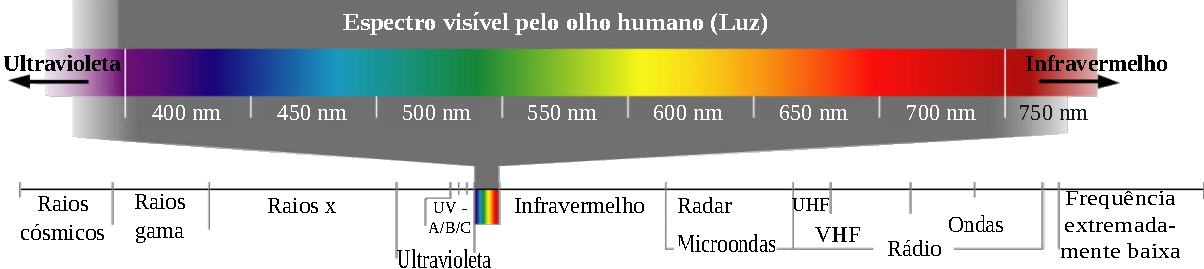
\includegraphics[scale=0.77]{_fig/espectroEletromagnetico.pdf}
    \caption[Especto eletromagnético]{Especto eletromagnético. Adaptado de~\citeonline{Gonzalez2008}.}
    \label{figEspectroEletromagnetico}
\end{figure}

O olho humano contém dois tipos de células especializadas em detectar cores: os bastonetes e os cones.
Em particular, os cones são capazes de identificar certos comprimentos de ondas de acordo com três propriedades importantes da luz visível para a formação das cores: radiância, luminância e brilho~\cite{Gonzalez2008}.

 \begin{enumerate}
    \item \underline{Radiância:} Indica a quantidade total de energia que flui da fonte de luz, em \textit{watts},
    
     \item \underline{Luminância:} Medida em \textit{lumens}, indica a quantidade de energia que um observador percebe de uma fonte, e
    
     \item \underline{Brilho:} Descritor subjetivo, incorpora a noção acromática de \textit{intensidade}, um dos principais fatores da percepção das cores.
\end{enumerate}

A fim de quantificar as cores, pode-se fazer uso do padrão de cromaticidade estabelecido pela Comissão Internacional de Iluminação (CIE)\footnote{\url{www.cie.co.at/}}, ilustrado na Figura~\ref{figCIE}.
Esse diagrama representa inúmeras cores de acordo com a composição das coordenadas de cromaticidade do gráfico~\cite{Gonzalez2008}.

\begin{figure}[!htb]
    \centering
    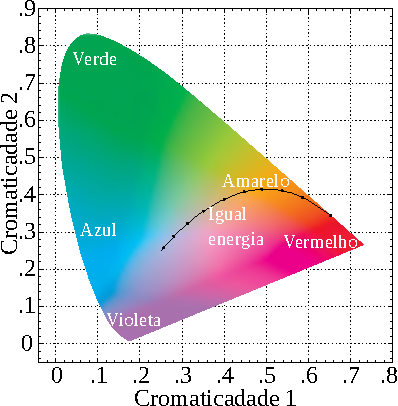
\includegraphics[scale=1]{_fig/cie.pdf}
    \caption[Diagrama de cromaticidade]{Diagrama de cromaticidade. Adaptado de~\citeonline{Gonzalez2008}.}
    \label{figCIE}
\end{figure}

\subsection{Modelos de cores}

Modelos de cores são uma especificação de coordenadas que delimitam um subespaço no padrão CIE, com o objetivo de representar cada cor como um ponto~\cite{Sonka1993}.
Os modelos de interesse desse trabalho são: RGB, HSI e LAB.

\subsubsection{Modelo RGB}

Este modelo de cores utiliza um espaço tridimensional, com a finalidade de representar as cores em três dimensões, denominadas vermelho, verde e azul (Figura~\ref{figModeloDeCores}(a)). 
Todas as cores nesse modelo têm a propriedade de serem representadas como uma composição vetorial, onde se emprega a combinação dos eixos vermelho, verde e azul para a geração de todas as cores. 
Os pontos nesse espaço tridimensional, além de formarem cores visíveis também podem ser vistos como a estrutura de dados denominada \textit{pixel}.
Um pixel é a estrutura de dados que corresponde a unidade \textit{atômica} de uma imagem digital~\cite{mccamy1976,Sonka1993}, de acordo com a Definição~\ref{def:pixel}.

\begin{definition}\label{def:pixel}[Pixel] 
Um pixel $P_i=\{r_i,g_i,b_i\} $ é constituído por uma tupla no espaço de cores RGB, onde $r_i$ é a componente do eixo vermelho, $g_i$ é a componente do eixo verde e $b_i$ é a componente do eixo azul.
\end{definition}

A \textit{profundidade} do pixel está computacionalmente associada ao número de cores gerados por esse modelo, medida em termos do número de bits $b$ que são empregados para retratar cada componente vetorial. 
A representação de uma imagem em padrões conhecidos se dá normalmente por oito bits de profundidade, como nos padrões JPEG, descrito por~\citeonline{Ahmed1974}, e PNG, detalhado por~\citeonline{Boutell1997}.
Como os oito bits são definidos para cada camada, ao se multiplicar todas as três camadas obtém-se a profundidade total do pixel de 24-bits.
Imagens de 24-bits são denominadas \textit{full-color} e permitem a representação de $(2^8)^3 = 16.777.216$ cores distintas~\cite{Chang1996,Gonzalez2008}.  

\begin{figure}[!htb]
    \centering
    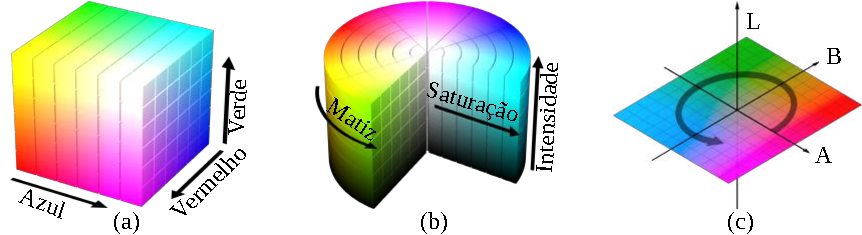
\includegraphics[scale=0.8]{_fig/modelocores.pdf}
    \caption[Modelos de cores]{Modelos de cores.
    (a)~Modelo RGB.
    (b)~Modelo HSI.
    (c)~Modelo LAB.
    Adaptado de~\citeonline{Gonzalez2008}.}
    \label{figModeloDeCores}
\end{figure}

\subsubsection{Modelo HSI}

O modelo RGB se inspira no sistema visual humano ao buscar representar a forma na qual as células do olho percebem as cores. 
Contudo, esse modelo pode não ser adequado para descrever as cores de objetos, em termos de interpretação da luz visível, pois associa cores a uma combinação vetorial.
Por outro lado, o modelo HSI ilustra as tonalidades como matiz, saturação e intensidade e permite a descrever a luz visível~\cite{Gonzalez2008}.
Os componentes do modelo são:

\begin{itemize}
    
    \item \underline{Hue (Matiz):} Atributo associado ao comprimento de onda dominante dentro da mistura da luz. 
    A matiz representa a cor percebida pelo observador. 
    Ao se mencionar as cores, \textit{i.e.} vermelho ou amarelo, normalmente tem-se a referência à matiz. 
    
    \item \underline{Saturação:} Refere-se à (ausência da) quantidade de luz branca que compõe a matiz.
    As cores denominada puras, são totalmente saturadas e possuem a combinação de cores da matiz e luz branca.
    Por exemplo, ``cor-de-rosa'' pode ser a combinação de ``vermelho'' com ``branco''.
    O grau de saturação é inversamente proporcional a quantidade de luz branca adicionada a uma cor qualquer.
    
    \item \underline{Intensidade:} Incorpora a noção acromática de intensidade, isto é, uma propriedade para permitir descrever a ``sensação'' das cores. 
\end{itemize}

Ao contrário do modelo de cores RGB, o HSI é expresso no formato de um cilindro vertical.
Na base do cilindro ficam as cores escuras e no topo ficam as cores mais claras.
O eixo da Matiz representa as cores em coordenadas polares em planos ortogonais, ou seja, as cores são localizadas em setores. 
Quanto mais distante do centro do cilindro, mais puras em matiz são as cores.
O eixo da Saturação possui propriedades semelhantes ao eixo da Matiz e as cores mais próximas a borda do cilindro são mais saturadas. 
A representação do modelo HSI é ilustrado na Figura~\ref{figModeloDeCores}(b).
Por último, mas não menos importante, destaca-se que é possível converter uma tonalidade de cor no espaço RGB para HSI e vice-versa, de acordo com a conveniência de cada representação.
A Definição~\ref{def:hsv2rgb} apresenta uma conversão pixel-a-pixel entre os dois modelos.

\begin{definition}\label{def:hsv2rgb}[Conversão RGB para HSI]
Um pixel $P_i$ definido no espaço RGB pode ser representado em um espaço HSI por meio de uma transformação geométrica.
Assumindo que o pixel $P_i$ tenha valores \textit{normalizados}, ou seja, que as coordenadas estejam no intervalo $[0,1]$, as dimensões $h_i$ (matiz), $s_i$ (saturação) e $v_i$ (intensidade) de $P_i$ são dadas pela Equação~\eqref{eqH:rgb2hsv}:
\begin{equation} \label{eqH:rgb2hsv}
\begin{split}
h_i = 
\left \{ 
\begin{matrix} 
    \cos{^{-1}} 
    \left \{ 
    \begin{matrix} 
        \frac 
            {\frac{1}{2} ~ [ (r_i - g_i) + ( r_i - b_i ) }
            {[r_i - b_i ]^2 + (r_i - b_i) (g_i - b_i) ^ { \frac{1}{2} } }
    \end{matrix} 
    \right.
    \quad \quad \quad \: \text{se } b_i  \leq  g_i 
    \\ 
    360 - 
    \cos{^{-1}} 
    \left \{ 
    \begin{matrix} 
        \frac 
            {\frac{1}{2} ~ [ (r_i - g_i) + ( r_i - b_i ) }
            {[r_i - b_i ]^2 + (r_i - b_i) (g_i - b_i) ^ { \frac{1}{2} } }
    \end{matrix} 
    \right.
    \quad \text{se} \: b_i > g_i
\end{matrix} 
\right.
\\
s_i = 1 - \frac{3}{(r_i + g_i + b_i)} ~ [min(r_i, g_i ,b_i)]
\\
v_i =  \frac{1}{3} ~ (r_i + g_i + b_i)
\end{split}
\end{equation}
\end{definition}


O modelo HSI de cores permite interpretar a luz visível, mas não é geometricamente \textit{``uniforme"}, no sentido que uma mesma distância euclideana nesse espaço não representa a diferença proporcional perceptível entre os estímulos de cores. 
O CIE estabelece um outro modelo, o LAB, para representar cores em um espaço quase uniforme~\cite{Connolly1997}.

\subsubsection{Modelo LAB}

Este modelo de cores preza por gerar um espaço com alto nível de consistência das cores do diagrama CIE, independentemente do instrumento de projeção~\cite{johnson2003}. 
O modelo se baseia na premissa de cores opostas com três pilares. 
O primeiro pilar apresenta, a luminosidade (L), enquanto os outros indicam cores diametralmente opostas(A e B) em um plano de coordenadas cromáticas. 
De forma mais detalhada, \citeonline{zhang1996} define as coordenadas LAB como:

\begin{itemize}

    \item \underline{L}: Representa a luminosidade, ou seja, descreve a intensidade da cor.
    
    \item \underline{A}: Apresenta o valor dos eixo das cores opostas. 
    Em um plano base (sem intensidade), essas cores são vermelha e verde, pois o eixo começa na cor vermelha e se torna verde conforme se aproxima do final. 

    \item \underline{B}: Corresponde as cores amarela e azul em um único eixo.
    Em um plano base (sem intensidade), essas cores são amarelo e azul.
\end{itemize}

A ilustração do modelo LAB é apresentado como uma sequência de planos na Figura~\ref{figModeloDeCores}(c).
Ao contrário da conversão RGB para HSI, a conversão de um pixel do espaço RGB para o modelo LAB é uma sequência de duas transformações que incluem uma base intermediária, como na Definição~\ref{def:rgb2lab}.

\begin{definition}\label{def:rgb2lab}[Conversão RGB para LAB]
Um pixel $P_i$ representado no espaço RGB unitário é representado no espaço LAB por intermédio de duas transformações: primeiro ao espaço XYZ e deste para o LAB, gerando as componentes $L_i$, $A_i$ e $B_i$ de acordo com a Equação~\eqref{eq:rgb2lab}. 
\begin{equation} \label{eq:rgb2lab}
\begin{split}
\begin{bmatrix}
    x_i\\
    y_i\\
    z_i
\end{bmatrix}
=
\begin{bmatrix}
    0,4124 & 0,3576 & 0,1805 \\
    0,2126 & 0,7152 & 0,0722 \\
    0,0193 & 0,1192 & 0,9505
\end{bmatrix}
\cdot
\begin{bmatrix}
    r_i\\
    g_i\\
    b_i
\end{bmatrix}
\\
L_i = 116*f\left(\frac{y_i}{100}\right) - 16,\\
A_i = 500*f\left(\frac{x_i}{95,047} - \frac{y_i}{100}\right), \\
B_i = 200*f\left(\frac{y_i}{100} - \frac{z_i}{108,883}\right),\\
f(k) =
\begin{cases}
    \sqrt[3]{k},     & \text{se } k > (6/29)^3 \\
    \frac{k}{3*(6/29)^2} + \frac{4}{29}\,   & \text{caso contrário}
\end{cases},
\end{split}
\end{equation} 

\end{definition}

\subsection{Imagem Digital}

Uma imagem digital $I$ é um conjunto ordenado de pixels $ I = \{P_i ~ | ~ 0 \leq i <n \}$, onde $n$ é o número total de pixels.
Caso um pixel $P_i$ tenha as três dimensões RGB equivalentes em valor, \textit{i.e.}, $r_i = g_i = b_i$, o pixel é dito \textit{unidimensional}.
Se todos os pixels $P_i$ de uma imagem $I$ forem unidimensionais, então a imagem é dita \textit{monocromática}, apresenta aspecto visual de tons de cinza, e pode ser representado por apenas \textit{um único valor} das quaisquer três dimensões do sistema RGB~\cite{Sonka1993,johnson2003,Chang1996}.
\citeonline{Gonzalez2008} definem as áreas de interesse para o processamento de imagens digitais em RGB ou monocromáticas em três níveis:

\begin{enumerate}
    \item \textbf{Processo de baixo nível.}
    As operações primitivas do pré-processamentos de imagens visam realçá-las, aumentando o contraste, nitidez, brilho e ruídos.
    Para  isso se empregam  técnicas de transformações de tonalidade, filtragens espaciais e no domínio da frequência. 
    Esse processo recebe uma imagem como entrada e também retorna uma única imagem. 
    
    \item \textbf{Processo de médio nível.}
    Caracterizado por tarefas de segmentação, o processo possui como objetivo descartar partes irrelevantes de uma imagem.
    Rotinas desse nível recebem uma imagem de entrada e geram uma ou mais imagens de saída.
    
    \item \textbf{Processo de alto nível.}
    Buscam encontrar \textit{significados} nas imagens, o que pode incluir técnicas de aprendizado de máquina para buscar determinados padrões, que podem ser representados por similaridades dentre e entre imagens.
\end{enumerate}

Neste trabalho final de curso, abordaremos todos os três processos. 
Para o primeiro processo utilizaremos técnicas de filtragens.
Já para o segundo processo, usaremos métodos de classificação para segmentar o fundo da imagem.
Finalmente, no terceiro processo empregaremos algoritmos de agrupamento para unir padrões de tecidos em imagens de úlceras venosas.

\subsubsection{Filtro da mediana}

O filtro de mediana realiza a \textit{normalização} de pixels em uma determinada vizinhança através da mediana.
Os valores dos pixels vizinhos são ordenados e o valor do pixel consultado é substituído, como exemplificado na Figura~\ref{fig:filtro_mediana}.

\begin{figure}[!htb]
    \centering
\centering
\vspace{-5px}
\begin{tabular}{
>{\columncolor[HTML]{EFEFEF}}c |
>{\columncolor[HTML]{EFEFEF}}c |
>{\columncolor[HTML]{EFEFEF}}c |
>{\columncolor[HTML]{CBCEFB}}c |
>{\columncolor[HTML]{EFEFEF}}c |
>{\columncolor[HTML]{EFEFEF}}c |
>{\columncolor[HTML]{EFEFEF}}c }
143 & 110 & 146 & \cellcolor[HTML]{C0C0C0} & 143 & 110 & 146 \\ \cline{1-3} \cline{5-7} 
105 & \cellcolor[HTML]{C0C0C0}249 & 208 & \cellcolor[HTML]{EFEFEF} & 105 & \cellcolor[HTML]{C0C0C0}208 & 208 \\ \cline{1-3} \cline{5-7} 
229 & 240 & 239 & \multirow{-3}{*}{\cellcolor[HTML]{C0C0C0}$\implies$} & 229 & 240 & 239 \\ \hline
\multicolumn{3}{c|}{(a)} & \cellcolor[HTML]{FFFFFF} & \multicolumn{3}{c}{(b)}
\end{tabular}
    \caption[Exemplo da aplicação do filtro da mediana.]{Exemplo da aplicação do filtro da mediana para uma imagem em (a) e uma vizinhança de $3\times3$ para o pixel unidimensional $(1,1) = 249$.
    Tem-se que os vizinhos de (a) são: 143, 110, 146, 105, 208, 229, 240, 239 além do próprio 249.
    A mediana desses valores é 208.
    A imagem resultante (b) tem o pixel com os valores atualizados.
    As bordas não foram alteradas pois não há ``encaixe'' da janela de vizinhança de $3\times3$.
    }
    \label{fig:filtro_mediana}
\end{figure}

O filtro da mediana é um filtro estatístico que tem como objetivo descartar valores de \textit{pixels} discrepantes em $I$.
Portanto, o filtro altera os valores dos pixels unidimensionais baseados em uma janela de vizinhança~\cite{Sun1994}.
A extensão do filtro da mediana para pixels não unidimensionais é simples: basta se calcular a mediana para cada uma das três dimensões, sejam elas RGB, HSI ou LAB, em separado.

\subsubsection{Método de Otsu}

O método de Otsu é um algoritmo de limiarização que respeita a frequência dos valores de pixels de uma imagem.
A abordagem é usualmente empregada para imagens monocromáticas, mas pode ser estendida para imagens \textit{full-color}.
A técnica depende da definição de um \textit{threshold} (ponto de corte) ideal para transformar uma imagem monocromática em uma imagem de dois tons (binária).
Essa definição é feita utilizando o histograma de tons de cinza da imagem monocromática~\cite{Otsu1979,Zhu2009}.

Um histograma representa uma distribuição de frequência para um conjunto de valores (no caso da imagens monocromáticas, os valores são os tons de cinza)~\cite{Kapur1985}. 
Esses valores podem ser representados em um conjunto de inteiros delimitado no intervalo $[1, 2, \cdots, 2^b]$, onde $2^b$ representa a profundidade do valor do pixel unidimensional em bits.
Para uma imagem $I$, a frequência acumulada no histograma é igual a quantidade $n$ de pixels.

\begin{algorithm} [!b]
\nonl \rule[0.5ex]{410px}{0.5pt}\\


\SetKwInOut{Input}{Entrada}
\SetKwInOut{Output}{Saída}

\Input{Imagem monocromática $I$, \textit{threshold} $\tau$}
\Output{Imagem binária $I'$}
\nonl \rule[0.5ex]{410px}{0.5pt}\\
$I' \leftarrow \emptyset$;
$tMax \leftarrow -1$;
$varMax \leftarrow -1$; $H \leftarrow$ calcularHistograma$(I)$ \;

\For{$t  \in [1, 2, \cdots, 2^b]$}  {
    $\mu_1 \leftarrow$ media($H \leq t$);
    $\sigma^2_1 \leftarrow$ variancia($\mu_1, H \leq t$)\;
    $\mu_2 \leftarrow$ media($H > t$);
    $\sigma^2_2 \leftarrow$ variancia($\mu_2, H > t$)\;

    \If{varianciaEntreHistogramas($H, \mu_1, \sigma^2_1, \mu_2, \sigma^2_2, t$) $> varMax$} {
        $varMax \leftarrow$ varianciaEntreHistogramas($H, \mu_1, \sigma^2_1, \mu_2, \sigma^2_2, t$)\;
        $\tau \leftarrow t$ \;
    }
}
\For {$P_i \in I$} {
            \eIf{$r_i = g_i = b_i \leq \tau$} { 
                $P_i \leftarrow (1,1,1)$
            } { $P_i \leftarrow (0,0,0)$  }
            $I' \leftarrow I' \cup P_i$\;
}
\Return $I'$\;
\nonl \rule[0.5ex]{410px}{0.5pt}\\
\caption{Método de limiarização de Otsu.}\label{alg:otsu}
\end{algorithm}

O histograma permite calcular o \textit{threshold} $\tau$ encarregado dividir (ou \textit{binarizar}) os pixels em dois grupos: $C_0$ e $C_1$~\cite{Sheng2005}.
O grupo $C_0$ será transformado em um único tom claro ($0$) e o grupo $C_1$ será transformado em um único escuro ($1$).
O cálculo da frequência de cada tonalidade $t$ gera um vetor com a quantidade de pixels cujo valor unidimensional seja igual a $t, t~\in [1, 2, \cdots, 2^b]$.
A escolha do \textit{threshold} $\tau$ é feita iterativamente.
Para cada iteração divide-se o histograma em duas partes, utilizando um valor candidato $t$ para $\tau$ no intervalo $[1, 2, \cdots, 2^b]$.
Calcula-se uma média $\mu_1$ e uma variância $\sigma^2_1$ para o histograma de pixels cujo valor de tonalidade seja menor ou igual a $t$ e uma segunda média $\mu_2$ e variância $\sigma^2_2$ para o histograma de pixels cujo valor unidimensional seja maior que $t$.
Se a variância entre os dois histogramas, calculada a partir das médias e variâncias $1$ e $2$, é a maior até o momento, então $t$ é escolhido como o melhor candidato até essa iteração.
Ao final das $2^b$ iterações, o $t$ de maior variância entre os dois histogramas é escolhido como o threshold $\tau$.

Seja uma imagem monocromática $I$, um histograma $H$ construído para os valores $t \in [1, 2,$ $\cdots, 2^b]$ e frequências de $P_i \in I$, o Algoritmo~\ref{alg:otsu} resume o método de limiarização de Otsu.

\subsubsection{Morfologia Matemática}

As operações morfológicas contemplam a segunda fase de processamento de imagens com o objetivo de encontrar objetos específicos nas imagens.
Esses objetos são figuras geométricas, denominadas de elementos estruturantes (SE)~\cite{Zhang2011}, que são uma pequena imagem a ser casada múltiplas vezes sobre a imagem processada como uma janela deslizante.
O formato e os pixels de cada elemento estruturante é personalizado de acordo com aplicação ou contexto da imagem~\cite{Gonzalez2008}.
A Figura~\ref{figWirebond} ilustra exemplos de duas operações morfológicas em uma imagem binária. 
No exemplo, a imagem original (Figura~\ref{figWirebond}(a)) tem o tamanho de $486 \times 486$ pixels e o Elemento Estruturante SE é um quadrado completo de pixels brancos de tamanho $11 \times 11$.\\

\noindent
\textbf{Dilatação.}
A dilatação é um processo complementar a erosão, com o objetivo de expandir determinados objetos de uma imagem.
Os processos de erosão e dilatação são semelhantes, pois combinam um elemento estruturante a uma imagem~\cite{Sonka1993}.
Uma dilatação soma o elemento estruturante SE como uma janela sobre uma imagem binária $I$ resultando em uma imagem $I'$, \textit{i.e.}, $I' = I ~\oplus$ SE.
Na operação de soma, caso o pixel esteja contido na janela deslizante, então o valor do pixel se propaga para sua borda.
Um exemplo de dilatação é ilustrado na Figura~\ref{figWirebond}(b), onde as linhas foram dilatas por um elemento quadrado de pixels brancos de tamanho $11 \times 11$ e a imagem original está ilustrada na Figura~\ref{figWirebond}(a).\\

\noindent
\textbf{Erosão.}
Seja uma imagem binária $I$ é um elemento estruturante SE, ao se empregar a subtração de \textit{I} por SE com o auxílio de uma janela deslizante sobre todos os pixels de $i$ se obtém uma terceira imagem $I'$.
A operação de subtração é denotada por $\ominus$ e, portanto, $I' = I ~\ominus$ SE.
A erosão remove componentes que não estão contidos no intervalo de valores delimitado por SE. 
Visualmente, os valores restantes sofrem um \textit{``afinamento"}~em suas bordas.
A Figura~\ref{figWirebond}(c) ilustra a erosão da imagem original da Figura~\ref{figWirebond}(a) por um elemento estruturante quadrado de pixels brancos de tamanho $11 \times 11$.\\

Ressalta-se que as operações morfológicas de dilatação e erosão são complementares, de maneira que aplicar a dilatação seguida por uma erosão com mesmo elemento estruturante gera a técnica conhecida como \textit{abertura}.
No entanto, caso a ordem da aplicação seja invertida o resultado da operação é diferente, o que gera a técnica conhecida como \textit{fechamento}~\cite{Sonka1993}.\\

\noindent
\textbf{Abertura.} 
O propósito desta operação morfológica é eliminar objetos de uma imagem e suavizar contornos dos objetivos restantes.
O método de abertura sobre uma imagem binária $I$ por SE, denotado por $\circ$, pode ser simplificado como
$I~\circ$ SE $ = (I~\ominus $ SE $)~\oplus$ SE.\\

\noindent
\textbf{Fechamento.}
A operação morfológica de fechamento busca restabelecer conexões entre objetos sem modificar radicalmente o tamanho e a forma dos conjuntos iniciais~\cite{Gil2002}.
O método de abertura sobre uma imagem binária $I$ por SE, denotado por $\bullet$, pode ser simplificado como
$I~\bullet$ SE $ = (I~\oplus $ SE $)~\ominus$ SE.

\subsubsection{Superpixels}

Superpixels são aglomerações de pixels em regiões de bordas visualmente bem definidas.
Portanto, superpixels constituem uma estratégia de processamento de imagens de médio nível, onde, para cada imagem de entrada são obtidas diversas imagens de saída que, potencialmente, representam objetos individuais.
A Definição~\ref{def:superpixel} formaliza o conceito de superpixel.

\begin{definition}\label{def:superpixel}[Superpixel]
Um superpixel $S$ corresponde a um conjunto ordenado de pixels $S \subseteq I$ definido com $S = \{P_{j} ~|~ 0 \leq j < m \}$, onde $m ~(m \leq n)$ é o número de pixels dentro do superpixel $S$. 
O valor médio, ou \textit{extraído}, de um superpixel é dado por um tupla $\bar{P_S}, \bar{P_S} = \langle \mu(s_1), \mu(s_2), \mu(s_3)\rangle$, onde $\mu(k) = \sum_{j = 0}^{m-1} k_j/m$, representando a média de valores dos pixels de $S$ em um espaço de cor de três dimensões arbitrários, \textit{i.e.}, RGB, HSI ou LAB.
O conjunto de superpixels extraídos de uma imagem $I$ é denotado por $\mathcal{S}$.
\end{definition}

Um algoritmo de geração de superpixels inicia como uma estrutura rígida de \textit{grade} de pixels que se moldam as bordas de acordo com a semelhança entre os pixels.
Esses algoritmos podem ser baseados em soluções derivadas de grafos ou cálculo de gradiente sobre um modelo de cor~\cite{Felzenszwalb2004,Vedaldi2008}.
De forma geral, esses métodos são funções $g(I, K_p) = \{S_j ~|~ 0 \leq j < K_p\}$ que usam uma imagem $I$ e geram $K_p$ superpixels disjuntos e não-vazios $S_j, ~S_j \subset I$.
A pesquisa comparativa empírica de~\citeonline{Achanta2012} avalia diversos métodos de geração de superpixels, incluindo:

\begin{itemize}
    
    \item \underline{TP09:} A técnica \textit{Turbopixel} dilata progressivamente um conjunto de sementes usando o fluxo geométrico de gradientes da imagem.
    
    \item \underline{NC05:} O método particiona, recursivamente, um grafo de todos os pixels da imagem usando pistas de contorno e textura, minimizando globalmente uma função de custo definida nas bordas nos limites da partição.
    
    \item \underline{GCa10 e GCb10: } O agrupamento dos superpixels é feito pela mescla de pixels da imagem, que são sobrepostos de forma que cada pixel pertença a apenas uma região. 
    A diferença entre as duas variantes (GCa10 e GCb10) é que o GCa10 gera superpixels mais compactos por intensidade de cor.
    
    \item \underline{QS09:} A técnica \textit{QuickShift} escolhe um pixel central para o agrupamento e move os pixels adjacentes recursivamente para aumentar a densidade de Parzen.
    
    \item \underline{GS04:} Realiza um agrupamento aglomerativo de pixels como nós em um grafo, de modo que cada superpixel pode ser visto como a árvore geradora mínima dos pixels envolvidos.
    
    \item \underline{Squares:} Gera um \textit{grid} uniforme de superpixels.
    
    \item \underline{GSLIC:} Variação do método SLIC (descrito na sequência), tendo a medida de distância euclideana alterada para distância geodésica, que garante conectividade.
    
    \item \underline{ASLIC:} Variação do método SLIC (descrito na sequência), que adota a medida de distância euclideana \textit{normalizada} de acordo com o espaço de cores.
    
\end{itemize}


\noindent
\textbf{SLIC.}
O método SLIC se destaca graças a sua eficiência computacional e escalabilidade.
Isso se dá porque o SLIC otimiza o cálculo de distância entre os pixels dentro do superpixel e restringe a região de busca proporcionalmente ao tamanho do superpixel.

A implementação do SLIC requer apenas um único parâmetro para seu funcionamento: o número $k$ final de superpixels \textit{desejado}. 
Tendo por base o número $k$, o SLIC inicia a etapa de armazenamento dos pixels em grupos, começando com $k$ centros de grupos descritos no espaço LAB e escolhidos como os pontos centrais de um \textit{grade} regular e equi-espaçada sobre a figura.
A cada iteração, os centróides dos grupos são movidos para os locais cuja posição do gradiente de cor LAB seja a mais baixa de todo o superpixel.
Assim, cada pixel é atribuído ao centróide mais próximo no espaço LAB, sendo que apenas centróides que estejam dentro de um limiar de distância de localização na imagem são considerados como candidatos.
Essa limiarização é fundamental para melhorar a velocidade de processamento do algoritmo, em virtude de restringir um limite para busca por centróides candidatos.
O limiar é calculado dinamicamente em função da área de cada superpixel e da totalidade da área da imagem.

Quando todos os pixel tiverem sido associados aos seus respectivos grupos, os centróides são atualizados novamente e um erro residual é calculado considerando-se as posições atuais e anteriores dos centróides no espaço LAB.
O processo de atribuição e atualização de centróides se repete até a convergência do erro residual.
Por último, o SLIC faz um pós-processamento que impõe conectividade para os superpixels ao unir os pixels separados em grupos pequenos aos superpixels próximos~\cite{Achanta2012}.

\begin{figure}[!t]
\centering
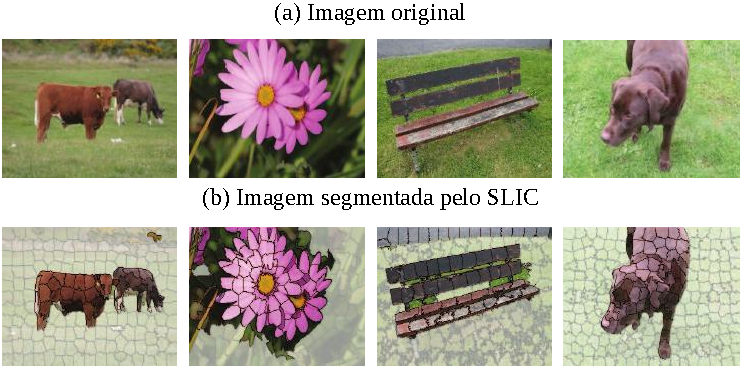
\includegraphics[scale=1]{_fig/ie_slic.pdf}
\vspace{-8px}
\caption[Exemplo de superpixels gerados pelo método SLIC]{Exemplo de superpixels gerados pelo método SLIC.
Adaptado de~\citeonline{Achanta2012}.}
\label{fig:ie_slic}
\end{figure}

\subsection{Aprendizado de Máquina}

A finalidade do aprendizado de máquina (AM) é encontrar padrões através da análise dos dados via algoritmos de tomada de decisão que não são explicitamente programados como um programa tradicional~\cite{Sullivan2017}.
De fato, diversos autores buscam \textit{separar} a programação tradicional e AM, como \citeonline{Sullivan2017}:

\begin{itemize}
    \item \underline{Programação tradicional}: Recebe dados que serão processados de forma determinística ou com um (ou mais) fluxo de ações pré-definido pelo programador. 
    Em suma, pode ser descrito como um programa que possui entrada e saída. 
    
    \item \underline{Aprendizado de Máquina}: Algoritmo genérico, que se torna especializado na tomada de decisão com base em um conjunto de dados previamente fornecido para sua especialização.  
    Ao contrário da programação tradicional, o algoritmo de AM recebe diversos dados e tenta encontrar padrões relevantes para o conjunto e não, necessariamente, para um domínio genérico.
    O comportamento do processamento é determinado em boa parte pelos dados e não apenas por um fluxo de programação. 
    A Figura~\ref{fig:class} mostra um algoritmo de AM, com viés de aprendizado linear, que encontrou uma fronteira de decisão para um conjunto de dados de duas classes.

\end{itemize}

Em específico, AM apresenta dois paradigmas fundamentais para a detecção de padrões em conjuntos de dados, a saber: supervisionado e não supervisionado~\cite{Bonaccorso2018}.
Esses paradigmas podem ser melhor detalhados como:

\begin{itemize}
    \item \underline{Supervisionado}: 
    Aprendizado indutivo, onde a análise é feita sobre coleções de dados rotuladas.
    O algoritmo de aprendizado terá que realizar classificação.
    O aprendizado supervisionado apresenta duas fases: treinamento e teste.
    A fase de treinamento consiste em detectar padrões correlacionados aos rótulos, enquanto a fase de teste usa esses padrões para rotular novos dados desconhecidos que são apresentados para classificação.
    As métricas de qualidade obtidas pelos diferentes algoritmos dependem do resultado do classificador em acertar os rótulos.  

    \item \underline{Não supervisionado}: 
    Possui o objetivo de identificar propriedades de dados que não apresentam rótulos.
    Rotular conjuntos de dados com alta precisão, muitas vezes é uma tarefa dispendiosa ou infactível, razão pela qual identificar padrões sem auxílio de classificação é tão importante.
    Algoritmos não supervisionados geralmente demandam conjuntos de maior \textit{cardinalidade} (número de entradas, ou \textit{instâncias}, do conjunto de dados) que os supervisionados~\cite{hastie2009}.
\end{itemize}

    \begin{figure}[!t]
    \centering
    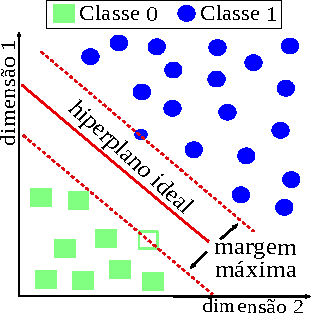
\includegraphics[scale=1]{_fig/class.pdf}
    \caption[Exemplo de fronteira de decisão para duas classes]{Exemplo de fronteira de decisão para duas classes. 
    Todos os objetos que estiverem acima da linha serão classificados como Classe~0 e os abaixo da linha como Classe~1. 
    Adaptado de \citeonline{Wang2005}.}
    \label{fig:class}
    \end{figure}

\subsubsection{Classificação de Dados}

Um classificador busca rotular dados a partir de um viés de aprendizado e um conjunto rotulado de exemplos.
No caso desse trabalho, os dados são pedaços das imagens -- superpixels, ou suas unidades atômicas -- pixels, que podem ser rotulados por um especialista do domínio, \textit{i.e.}, dermatologista, ou por um biomarcador, \textit{i.e.}, análise de biópsia em laboratório.
A Definição~\ref{def:classificador} formaliza o conceito de um classificador como uma função cujo comportamento depende do conjunto de dados de entrada desse tipo.

\begin{definition}\label{def:classificador}[Classificador]
Um classificador $\phi$ é uma função $\phi : \{\mathcal{P}, T\} \rightarrow L$, onde $L$ é um conjunto discreto e disjunto de rótulos, $\mathcal{P}$ é o domínio dos pixels, \textit{i.e.}, RGB, HSI ou LAB, e $T$ é o conjunto de treinamento que condiciona o comportamento de $\phi$.
Em particular, dado o domínio $\mathcal{P}$, $T$ representa um conjunto finito e não-vazio de pixels rotulados, \textit{i.e.}, $T = \{\langle P_i, l_j \rangle~|~L = \cup_j l_j\}$, e o algoritmo de aprendizado do classificador é um método enviesado que define o comportamento de $\phi$ a partir de $T$.
\end{definition}

Diferentes viéses podem ser usados no algoritmo de aprendizagem para predizer rótulos, sendo que a literatura costuma dividí-los em categorias~\cite{Faceli2008}.
As categorias mais conhecidas são: simbólica, conexionista, bayesiana e por exemplos~\cite{Domingos2015,Bradley1997}, detalhadas na sequência. 

\begin{itemize}

    \item \underline{Simbólica:} Identifica padrões por meio de estruturas simbólicas, \textit{i.e.}, árvores.
    Algoritmos desse paradigma incluem Decision~Tree~(DT), RandomForest~(RF) e RandomTree~(RT).
    
    \item \underline{Conexionista:}
    Inspirado na estrutura de aprendizagem cerebral, que é descrita por meio de ajustes das conexões entre os neurônios.
    Exemplos de algoritmos desse paradigma incluem as redes neurais artificiais Perceptron e Multi-Layer Perceptron (MLP).

    \item \underline{Bayesiana:} Busca identificar padrões por intermédio da probabilidade de ocorrência de uma classe conhecida.
    Tendo como exemplos de algoritmos desse paradigma incluem Na\"{i}ve-Bayes~(NB) e Bayes-Net~(BN).
    
    \item \underline{Por exemplos:} Possui o intuito de detectar padrões baseados em instâncias conhecidas. 
    Portanto, se baseia em calcular a semelhança de uma instância para outra.
    Exemplos de algoritmos desse paradigma são os \textit{k}-Vizinhos mais próximos (kNN) e Máquina de Vetores de Suporte (SVM).
\end{itemize}

Para se medir a qualidade de um classificador utiliza-se um outro conjunto de teste rotulado (diferente daquele empregado em seu treinamento) e solicita-se a classificação de cada instância desse segundo conjunto de forma individual.
Os acertos e os erros do classificador são anotados em uma matriz, denominada \textit{matriz de confusão}.
A Figura~\ref{fig:matriz_conf} apresenta um exemplo de matriz de confusão para um conjunto de dados que possui apenas dois rótulos $L = \{$Positivo,Negativo$\}$.
A matriz ilustra os índices de acerto e erro de um classificador, detalhando o que foi classificado como Positivo e realmente o é, denominado de Verdadeiro Positivo~(TP), e o Negativo que foi rotulado como Positivo, denominado Falso Positivo~(FP).
Além disso, a matriz indica os dados Positivos classificados como Negativos, os chamados Falso Negativos~(FN), e as instâncias Negativas realmente rotuladas como tal, os Verdadeiros Negativos (TN)~\cite{Townsend1971,Faceli2008,Aggarwal2015}.  

\begin{figure}[!htp]
    \centering
\begin{tabular}{l|c|c}
\cline{2-3}
\multicolumn{1}{c|}{}                    & 
\cellcolor[HTML]{CBCEFB}Real Positivo & \cellcolor[HTML]{CBCEFB}Real Negativo \\ \hline
\cellcolor[HTML]{CBCEFB}Predito Positivo & \cellcolor[HTML]{9AFF99}TP            & \cellcolor[HTML]{FD6864}FP            \\ \hline
\cellcolor[HTML]{CBCEFB}Predito Negativo & \cellcolor[HTML]{FD6864}FN            & \cellcolor[HTML]{9AFF99}TN            \\ \hline \hline
\end{tabular}
        \caption[Exemplo de matriz de confusão para duas classes]{Exemplo de matriz de confusão para duas classes $L = \{$Positivo,Negativo$\}$.}
    \label{fig:matriz_conf}
\end{figure}

Por intermédio da matriz de confusão pode-se obter diversos índices e métricas de qualidade que avaliam o desempenho dos classificadores~\cite{Congalton2008,Powers2011}.
Exemplos de métricas que usaremos na validação do trabalho proposta incluem:


\begin{itemize}
    \item 
    \underline{\textit{Revocação} ou \textit{Sensibilidade}:} 
    Mede a proporção de verdadeiros positivos (TP) com relação a todos os positivos.
    A Equação~\eqref{eq:recall} detalha essa métrica.

    \begin{equation} \label{eq:recall}
        \textit{Revocação} = Sensibilidade = \frac{TP}{TP + FN}
    \end{equation}
    
    \item  
    \underline{\textit{Precisão} ou \textit{Confiança}:} 
    Denota a proporção de verdadeiros positivos (TP) considerando todas as instâncias rotuladas como positivas.
    A Equação~\eqref{eq:precision} calcula essa métrica. 

    \begin{equation} \label{eq:precision}
         \textit{Precisão} = \textit{Confiança} =\frac{TP}{TP + FP}
    \end{equation}
    
    \item 
    \underline{\textit{Especificidade} ou \textit{Seletividade}:} 
    Mede a proporção de verdadeiros negativos (TN) com relação às instâncias preditas negativas.
    A Equação~\eqref{eq:specificity} apresenta a \textit{Especificidade}.  
    
    \begin{equation} \label{eq:specificity}
        \textit{Especificidade} =  \textit{Seletividade} = \frac{TN}{TN + FP}
    \end{equation}
    
    \item 
    \underline{\textit{Acurácia}:} 
    Mostra o acerto global do classificador como uma proporção de resultados verdadeiros entre o número total de casos examinados.
    A Equação~\eqref{eq:accuracy} apresenta essa métrica.
    
    \begin{equation} \label{eq:accuracy}
        \textit{Acurácia} = \frac{TN+TP}{TN + TP + FN + FP}
    \end{equation}

    \item 
    \underline{\textit{F-Measure}:} 
    Combinas as medidas de \textit{Precisão} e \textit{Revocação} em uma média harmônica, focada nos exemplos positivos e nas previsões corretas.
    A Equação~\ref{eq:fmeasure} detalha essa métrica.
    
    \begin{equation}\label{eq:fmeasure}
        \textit{\textit{F-Measure}} = 2 * \left( \frac{ \textit{Precisão} * \textit{Revocação}} { \textit{Precisão} + \textit{Revocação} } \right)
    \end{equation}
    
    \item 
    \underline{MSE e MAE:}
    Quantificam os acertos das previsões.
    O \textit{Mean Squared Error} (MSE) usa o erro quadrático médio e o \textit{Mean Absolute Error} (MAE) usa a diferença absoluta entre a classe real e a predita, tal qual nas Equações~\eqref{eq:mse} e \eqref{eq:mad}, que usam $\eta$ como o tamanho do conjunto de dados de teste. 
    
    \begin{equation} \label{eq:mse}
        \text{\textit{MSE}} =  \frac{1}{\eta} \sum^\eta_{i=1} (predita - real)^2
    \end{equation}
    
    \begin{equation} \label{eq:mad}
        \text{\textit{MAE}} =  \frac{1}{\eta} \sum^\eta_{i=1} |predita - real|
    \end{equation}
    
    \item 
    \underline{Coeficiente Cohen--Kappa:}
    Avalia os níveis de concordância entre dois conjuntos de rótulos, tal qual expresso na Equação~\ref{eq:ckc}.

    \begin{equation} \label{eq:ckc}
        \kappa = \left( \frac{\lambda_o - \lambda_e} {1 - \lambda_e} \right) =  1 - \left( \frac{1 - \lambda_o} {1 - \lambda_e} \right),
    \end{equation}

    onde $\lambda_o$ é a taxa de aceitação relativa e $\lambda_e$ simboliza a taxa hipotética de aceitação.
    Explicitamente, $\lambda_o = ( \frac{TP+TN}{\eta} )$ e $\lambda_e = (\frac{TP+FP}{\eta} \cdot \frac{TP+FN}{\eta}) + (\frac{FN+TN}{\eta} \cdot \frac{FP+TN}{\eta})$, $\eta$ sendo o tamanho do conjunto de testes.
    
\end{itemize}

O Coeficiente de Cohen-Kappa permite interpretar a qualidade de um classificador em termos semânticos~\cite{Sim2005}.
A Figura~\ref{fig:kappa} apresenta o intervalo de valores do Coeficiente de Cohen-Kappa associado ao nível de concordância semântica.

\begin{figure}[!htb]
    \centering
    \begin{tabular}{c|c}
\hline \hline  
\rowcolor[HTML]{C0C0C0} 
{\color[HTML]{000000} \textbf{Coeficiente de Kappa-Cohen}} & {\color[HTML]{000000} \textbf{Nível de Concordância}} \\ \hline \hline 
{\color[HTML]{000000} 0}                                   & {\color[HTML]{000000} Pobre}                          \\ \hline
\rowcolor[HTML]{EFEFEF} 
{\color[HTML]{000000} 0 – 0,20}                            & {\color[HTML]{000000} Leve}                           \\ \hline
{\color[HTML]{000000} 0,21 – 0,40}                         & {\color[HTML]{000000} Considerável}                   \\ \hline
\rowcolor[HTML]{EFEFEF} 
{\color[HTML]{000000} 0,41 – 0,60}                         & {\color[HTML]{000000} Moderada}                       \\ \hline
{\color[HTML]{000000} 0,61 – 0,80}                         & {\color[HTML]{000000} Substancial}                    \\ \hline
\rowcolor[HTML]{EFEFEF} 
{\color[HTML]{000000} 0,81 – 1}                            & {\color[HTML]{000000} Excelente} \\ \hline \hline 
\end{tabular}
        \caption[Nível de concordância do Coeficiente de Cohen--Kappa]{Nível de concordância do Coeficiente de Cohen--Kappa}
    \label{fig:kappa}
\end{figure}

Por último, \citeonline{Provost1998} argumenta que usar simplesmente um único valor de qualidade pode ser enganoso, recomendando também aplicar outras formas de avaliações, como a curva de Característica do Operador do Receptor~(ROC).
Essa curva ilustra como o número de exemplos positivos corretamente classificados varia de acordo com o número de exemplos negativos classificados incorretamente~\cite{Provost1998}.
A curva ROC utiliza as métricas de \textit{Revocação} e a \textit{Especificidade} para sua elaboração, onde cada ponto na curva ROC representa um par de \textit{Revocação} e \textit{Especificidade}.
Devido a essas diversas perspectivas de qualidade, nesse trabalho serão utilizados mais uma métrica de avaliação de classificação, de maneira, a evitar qualquer tipo de visão excessivamente otimista do desempenho de um classificador. 

\subsubsection{Redes Neurais Artificiais}

A proposta do Perceptron~\cite{Mcculloch1943} estabelece um modelo linear de classificação que recebe várias entradas e as processa por uma função linear.
No caso de um pixel $P_i$, as entradas são o valor da pixel em cada uma das dimensões que o descreve, \textit{e.g.}, $r_i$, $g_i$ e $b_i$.
Uma unidade que realiza a soma ponderada sobre cada entrada com pesos iniciais aleatórios é denominada \textit{neurônio} Perception.
Após o processamento por um neurônio há uma saída de valor real que pode ser convertida em binário, se conveniente ao domínio.
Caso o valor de saída não for o esperado, o neurônio pode ser \textit{treinado} ao se acrescentar ou diminuir o peso que ele atribui a cada entrada~\cite{Mcculloch1943,Rosenblatt1958}.

Redes neurais artificiais são evoluções/variações do Perceptron e possuem propriedades e componentes que as diferenciam entre si, tais como número de neurônios, sinapses, número de camadas, função de ativação e topologia. 
Esses aspectos podem ser detalhados como:

\begin{itemize}
    \item {\underline{Neurônio:}} Unidade que desempenha o processamento unitário da rede.
    Recebe várias entradas (dimensões) simultaneamente para cada instância, podendo transformá-las de acordo com uma função de ativação, e as associa com pesos, inicialmente aleatórios.
    Como resultado, obtém-se um único valor de saída, que pode ser usado como entrada para outros neurônios, caso exista uma ligação (sinapse) entre eles~\cite{Zhang1998,Aggarwal2015}.
    
    \item \underline{Sinapse:} Responsável por interligar neurônios e propagar entradas e saídas.
    As sinapses também são responsável de interligar as camadas da rede.

    \item \underline{Camadas:} Incluem um conjunto de neurônios e sinapses em uma determinada posição na topologia da rede, ou seja, uma camada é uma pequena rede neural artificial com neurônios paralelos.
    Algumas camadas possuem uma nomenclatura especial, como a 
    \textit{(i)}~camada de entrada, cuja quantidade de neurônios está, geralmente, associada ao número de dimensões que descrevem as instâncias,
    \textit{(ii)}~camada de saída, onde a quantidade de neurônios é geralmente, associado ao número de possíveis rótulos, e
    \textit{(iii)}~camadas ocultas, que estão entre a camada de entrada e a camada de saída~\cite{Hecht1988,Zhang1998}.
    
    \item \underline{Função de ativação:} Define a influência da dimensão na combinação linear com o peso. 
    Um exemplo de função de ativação é sigmóide logística, que fornece resultados no intervalo $[0,1]$~\cite{Lippmann1987,Jain1996}. 
    
    \item \underline{Topologia:} É a organização dos elementos da rede e a forma como os neurônios e camadas estão ligados.
    A Figura~\ref{fig:ann} ilustra um exemplo de topologia da uma rede MLP totalmente conectada.
    Toda topologia organiza a quantidade de camadas e a quantidade de neurônio, além de indicar quais desses neurônios se ligam a outros.
    Além disso, a topologia também indica qual o algoritmo de treinamento da rede, \textit{i.e.}, a estratégia a ser usada para ajustar os pesos inicialmente aleatórios~\cite{Kwok1997,Russell2016}.
 
\end{itemize}

\begin{figure}[!htb]
    \centering
    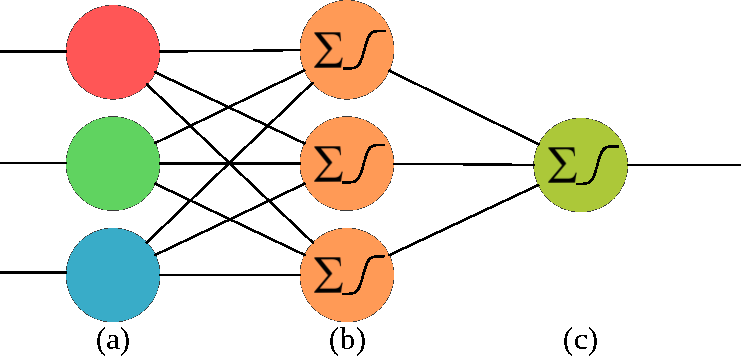
\includegraphics[scale=0.65]{_fig/ANN.pdf}
    \caption[Topologia de uma MLP totalmente conectada]{Topologia de uma MLP totalmente conectada.
    (a)~Camada de entrada.
    (b)~Camada oculta.
    (c)~Camada de saída. }
    \label{fig:ann}
\end{figure}

\noindent
\textbf{Treinamento.}
O treinamento de uma rede neural artificial é o ajuste dos pesos de seus neurônios.
Os dados (sem rótulos) são inseridos na camada de entrada e transmitidos para as camada ocultas por intermédio das sinapses até a camada de saída.  
O valor da saída é comparado com o rótulo real e, em caso de divergência, todos os pesos da rede são atualizados.
Os pesos começam com valores aleatórios entre $[0,1]$ e podem ser aumentados ou diminuídos a cada exemplo.

O ajuste dos pesos depende da conexão entre os neurônios na topologia da rede, que podem resultar em ajustes \textit{feedforward} e \textit{backpropagation}.
A Figura~\ref{fig:feedvsback} apresenta as duas diferentes conexões topológicas, sendo que a conexão \textit{backpropagation} inclui retroalimentação e é a mais utilizada~\cite{Faceli2008}.

\begin{figure}[!htb]
    \centering
    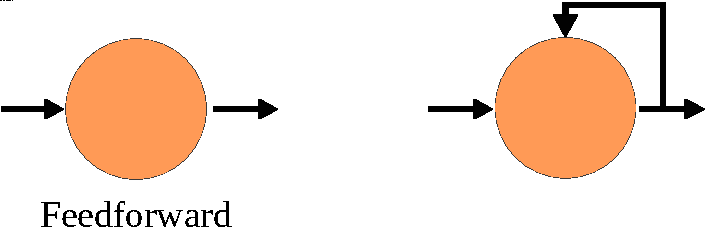
\includegraphics[scale=.6]{_fig/feedvsback.pdf}
    \caption[Conexão \textit{feedforward} e \textit{backpropagation}]{Conexão \textit{feedforward} e \textit{backpropagation}.}
    \label{fig:feedvsback}
\end{figure}

Dois métodos podem ser usados para ajuste de pesos com conexão com backpropagation: o \textit{Resilient Propagation} (RPROP) e a abordagem de Levenberg-Marquardt (LM)~\cite{Riedmiller2005,Cortez2002}.\\

\noindent
\textbf{Resilient-propagation -- RPROP.}
O método RPROP traz uma solução para as funções de ativação sigmóide ou tangente hiperbólica, que podem provocar a ocorrência da saturação da saída dos neurônios e gerar valores próximos de zero, o que influência a velocidade de convergência da rede neural artificial.
Em particular, a solução RPROP de \citeonline{Riedmiller2005} propõe atualizar os pesos considerando a variação do sinal do gradiente do erro ao invés das magnitudes do gradiente em si.\\

\noindent
\textbf{Levenberg-Marquardt -- LM.}
O método de Levenberg-Marquardt é uma aproximação do método de Newton e é uma alternativa para o custo computacional elevado da convergência do RPROP.
O algoritmo implementa um gradiente de segunda ordem, baseado no método dos mínimos quadrados para modelos não lineares~\cite{Suratgar2005,Yu2011}, o que permite treinar a rede em tempo menor que o do RPROP e com a mesma qualidade de resultado para topologias não muito grandes.

\subsubsection{Agrupamento de Dados}

Algoritmos de agrupamento de dados permitem analisar conjunto de dados não-rotulados~\cite{Jain1988}.
Esses métodos tem por objetivo dividir os dados em \textit{clusters} (grupos) de acordo com suas características.
Existem diversas abordagens e perspectivas de agrupamento~\cite{Faceli2008}, mas o foco desse trabalho é baseado em algoritmos de agrupamento particionais baseados em medidas de similaridade~\cite{Aggarwal2015,hastie2009}.
Nesse contexto, os dados são superpixels (ou pixels), identificados por três dimensões de acordo com o modelo de cores adotado e o algoritmo de agrupamento funciona como uma função dada pela Definição~\ref{def:agrupamento}.

\begin{definition}\label{def:agrupamento}[Agrupamento Particional]
Um método de agrupamento  particional é uma função $\theta$ que divide as entradas em um conjunto disjunto de grupos.
Dado um conjunto de superpixels $\mathcal{S}$ e um conjunto de grupos $\mathcal{C}$, o método de agrupamento $\theta: \mathcal{S} \rightarrow \mathcal{C}$ coloca cada superpixel $S \in \mathcal{S}$ em apenas um único grupo $C \in \mathcal{C}$ tal que $\cup_{C_i \in \mathcal{C}} C_i = \mathcal{S}$ e $\cap_{C_i \in \mathcal{C}} C_i = \emptyset$.
\end{definition}

A base para os algoritmos particionais desse tipo é medir a \textit{semelhança} entre dois elementos de dados, de acordo com sua representação multidimensional.
Uma modelagem eficiente para esse problema é a representação de similaridade por distâncias, por meio da Teoria de Espaços Métricos~\cite{Hetland2009}.
Uma função de distância é uma métrica de similaridade, com a intuição semântica de quanto maior a distância entre dois elementos de dados, mais dissimilares eles são.
A Definição~\ref{def:metrica} formaliza o conceito de função de distância métrica e a Definição~\ref{def:mink} apresenta a família Minkowski de distâncias que serão usadas no restante desse trabalho.

\begin{definition}\label{def:metrica}[Função de distância métrica]
Uma função de distância métrica $\delta$ é uma função $\delta: \mathbb{M} \times \mathbb{M} \rightarrow \mathbb{R}_{+}$ que mede a semelhança entre dois pontos em $\mathbb{M}$, \textit{i.e.}, coordenadas LAB.
Para quaisquer $m_1, m_2, m_3 \in \mathbb{M}$, $\delta$ satisfaz as seguintes propriedades: 
\textit{(i)}~simetria,
\textit{(ii)}~não-negatividade e  
\textit{(iii)}~desigualdade triangular.
\end{definition}

\begin{definition}\label{def:mink}[Família Minkowiski de funções -- $L_p$]
Dados dois elementos de dados $x$ e $y$ descritos em um espaço $d$-dimensional, \textit{i.e.}, $x, y \in \mathbb{R}^d$, uma função de Minkowski $L_p$ é uma função de distância métrica que calcula a similaridade entre $x$ e $y$ de acordo com a Equação~\ref{eq:mink}.
\begin{equation}\label{eq:mink}
    L_p = \left(\sum_{i = 1}^{d}\left(|x_i - y_i|^p\right)\right)^\frac{1}{p},
\end{equation}
para qualquer $p, p > 0$.
As funções de distâncias mais conhecidas de Minkowiski são as funções $L_1$ (City-Block), $L_2$ (Euclideana) e $L_\infty$ (Chebyshev).
\end{definition}

Além das funções de Minkowiski, outras métricas também são comumente empregadas como as funções Canberra e BrayCurtis~\cite{Hetland2009,Blanco2016}.
Ainda considerando  dois elementos de dados $x$ e $y$ descritos em um espaço $d$-dimensional, a distância de Canberra calcula a similaridade entre eles como expresso na Equação~\ref{eq:canberra}, enquanto a distância de Bray-Curtis usa a fórmula definida na Equação~\ref{eq:bray}.

\begin{equation}\label{eq:canberra}
    \delta(x, y) = \sum_{i = 1}^{d} \frac{|x_i - y_i|}{|x_i| + |y_i|}
\end{equation}
\begin{equation}\label{eq:bray}
    \delta(x, y) = 1 -  \frac{\sum_{i = 1}^{d}|x_i - y_i|}{\sum_{i = 1}^{d}x_i + \sum_{i = 1}^{d}y_i}
\end{equation}

De forma geral, um algoritmo de agrupamento particional irá colocar as instâncias mais similares em um mesmo grupo e tentará afastar os grupos.
Assim como para classificadores, diversas medidas de qualidade podem ser empregadas para medir a qualidade dos agrupamentos.\\

\noindent
\textbf{Medidas avaliativas.}
Ao contrário da matriz de confusão para classificadores, a qualidade dos métodos de agrupamento é mais subjetiva e depende, por vezes, da interferência humana (especialista do domínio).
De forma geral, três medidas de qualidade podem ser usadas para essa finalidade:

\begin{itemize}

\item \underline{Número de grupos:} 
Quando existe a noção de quantos grupos são esperados, essa medida pode auxiliar a indicar se a quantidade de grupos formados é adequado e se cada grupo constitui uma possível classe de dados.

\item \underline{Índices internos:} 
Verificam a qualidade da partição obtida sem considerar informações externas como um valor real.
O coeficiente de silhueta é um exemplo dessa medida.

\item \underline{Relativos:} 
Comparam dois grupos, utilizando de medidas orientadas a similaridade, como coesão intra grupos e separação inter grupos.
\end{itemize}

\subsubsection{DBSCAN}

\begin{figure}[!b]
\centering
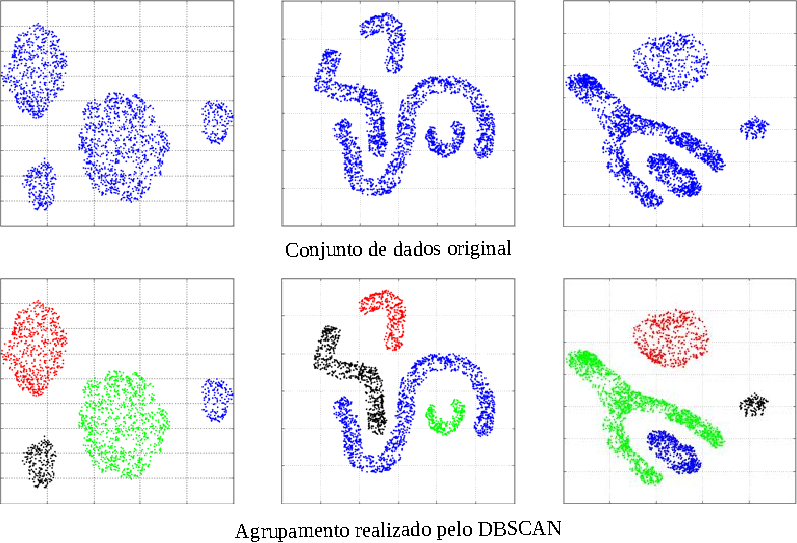
\includegraphics[scale=1]{_fig/dbscan.pdf}
\caption[Exemplos de formatos de agrupamento gerados pelo DBSCAN]{Exemplos de formatos de agrupamento gerados pelo DBSCAN.
Adaptado de~\citeonline{Mumtaz2010}.}
\label{fig:dbscan}
\end{figure}

O método DBSCAN (\textit{Density-Based Spatial Clustering of Applications with Noise}) é baseado na densidade de elementos por espaço, onde as instâncias do conjunto de dados são agrupados por similaridade.
Seguindo essa premissa, o algoritmo se destaca na detecção de grupos de formato arbitrário~\cite{Ester1996,Mumtaz2010}.
As propriedades de densidade são obtidas em função da distância máxima de similaridade, o que gera propriedades interessantes para espaços multidimensionais, como os exemplos na Figura~\ref{fig:dbscan}.
Entretanto, o método requer parâmetros externos para funcionar: a distância máxima de similaridade $\xi$ e o número mínimo de pontos aceitáveis para um grupo~\cite{Tan2007}.
De forma geral, uma partição gerada pelo DBSCAN tem as seguintes propriedades:

\begin{enumerate}
    \item Todos os pontos dentro do \textit{cluster} são mutuamente densamente conexos;
    \item Se um ponto é alcançável por densidade por algum ponto dentro de um \textit{cluster}, então ele também deve fazer parte do \textit{cluster}\footnote{Empates são quebrados arbitrariamente.}.
\end{enumerate}

A Figura~\ref{fig:ex_dbscan_passos} ilustra as iterações do algoritmo DBSCAN para a função de distância $\delta = L_2$, distância máxima $\xi = 2$ e um número mínimo de pontos por \textit{cluster} igual a dois.
A Tabela~\ref{tab:conjunto_dbscan} apresenta os pontos bidimensionais para demonstrar o método do DBSCAN, enquanto a Figura~\ref{fig:ex_dbscan_passos}(a) mostra os pontos bidimensionais em um gráfico.

\begin{table}[!htp]
\centering
\caption{Conjunto demonstrativo para o método do DBSCAN}
\label{tab:conjunto_dbscan}
\resizebox{.8\textwidth}{!}{%
\begin{tabular}{
>{\columncolor[HTML]{EFEFEF}}c |c|c|
>{\columncolor[HTML]{9B9B9B}}l |
>{\columncolor[HTML]{C0C0C0}}l |
>{\columncolor[HTML]{9B9B9B}}l |
>{\columncolor[HTML]{EFEFEF}}c |c|c}
\hline
\multicolumn{1}{l|}{\cellcolor[HTML]{DDDDDD}{\color[HTML]{000000} }} & \multicolumn{2}{l|}{\cellcolor[HTML]{DDDDDD}{\color[HTML]{000000} \textbf{Coordenada cartesiana}}}                    & {\color[HTML]{000000} } & {\color[HTML]{000000} } & {\color[HTML]{000000} } & \multicolumn{1}{l|}{\cellcolor[HTML]{DDDDDD}{\color[HTML]{000000} }} & \multicolumn{2}{l|}{\cellcolor[HTML]{DDDDDD}{\color[HTML]{000000} \textbf{Coordenada cartesiana}}}                    \\ \hline
{\color[HTML]{000000} \textbf{Elementos}}                            & \cellcolor[HTML]{EFEFEF}{\color[HTML]{000000} \textbf{X}} & \cellcolor[HTML]{EFEFEF}{\color[HTML]{000000} \textbf{Y}} & {\color[HTML]{000000} } & {\color[HTML]{000000} } & {\color[HTML]{000000} } & {\color[HTML]{000000} \textbf{Elementos}}                            & \cellcolor[HTML]{EFEFEF}{\color[HTML]{000000} \textbf{X}} & \cellcolor[HTML]{EFEFEF}{\color[HTML]{000000} \textbf{Y}} \\ \hline
{\color[HTML]{000000} \textbf{A}}                                    & \cellcolor[HTML]{FFFFFF}{\color[HTML]{000000} 0,05}       & \cellcolor[HTML]{FFFFFF}{\color[HTML]{000000} 0,40}       & {\color[HTML]{000000} } & {\color[HTML]{000000} } & {\color[HTML]{000000} } & {\color[HTML]{000000} \textbf{K}}                                    & {\color[HTML]{000000} 4,27}                               & {\color[HTML]{000000} 9,37}                               \\ \hline
{\color[HTML]{000000} \textbf{B}}                                    & \cellcolor[HTML]{FFFFFF}{\color[HTML]{000000} 0,18}       & \cellcolor[HTML]{FFFFFF}{\color[HTML]{000000} 1,29}       & {\color[HTML]{000000} } & {\color[HTML]{000000} } & {\color[HTML]{000000} } & {\color[HTML]{000000} \textbf{L}}                                    & {\color[HTML]{000000} 4,45}                               & {\color[HTML]{000000} 3,35}                               \\ \hline
{\color[HTML]{000000} \textbf{C}}                                    & \cellcolor[HTML]{FFFFFF}{\color[HTML]{000000} 0,99}       & \cellcolor[HTML]{FFFFFF}{\color[HTML]{000000} 8,80}       & {\color[HTML]{000000} } & {\color[HTML]{000000} } & {\color[HTML]{000000} } & {\color[HTML]{000000} \textbf{M}}                                    & {\color[HTML]{000000} 4,91}                               & {\color[HTML]{000000} 7,82}                               \\ \hline
{\color[HTML]{000000} \textbf{D}}                                    & \cellcolor[HTML]{FFFFFF}{\color[HTML]{000000} 1,15}       & \cellcolor[HTML]{FFFFFF}{\color[HTML]{000000} 2,27}       & {\color[HTML]{000000} } & {\color[HTML]{000000} } & {\color[HTML]{000000} } & {\color[HTML]{000000} \textbf{N}}                                    & {\color[HTML]{000000} 5,80}                               & {\color[HTML]{000000} 8,70}                               \\ \hline
{\color[HTML]{000000} \textbf{E}}                                    & \cellcolor[HTML]{FFFFFF}{\color[HTML]{000000} 1,45}       & \cellcolor[HTML]{FFFFFF}{\color[HTML]{000000} 9,32}       & {\color[HTML]{000000} } & {\color[HTML]{000000} } & {\color[HTML]{000000} } & {\color[HTML]{000000} \textbf{O}}                                    & {\color[HTML]{000000} 5,74}                               & {\color[HTML]{000000} 7,47}                               \\ \hline
{\color[HTML]{000000} \textbf{F}}                                    & \cellcolor[HTML]{FFFFFF}{\color[HTML]{000000} 1,85}       & \cellcolor[HTML]{FFFFFF}{\color[HTML]{000000} 0,29}       & {\color[HTML]{000000} } & {\color[HTML]{000000} } & {\color[HTML]{000000} } & {\color[HTML]{000000} \textbf{P}}                                    & {\color[HTML]{000000} 5,93}                               & {\color[HTML]{000000} 6,30}                               \\ \hline
{\color[HTML]{000000} \textbf{G}}                                    & \cellcolor[HTML]{FFFFFF}{\color[HTML]{000000} 3,38}       & \cellcolor[HTML]{FFFFFF}{\color[HTML]{000000} 7,39}       & {\color[HTML]{000000} } & {\color[HTML]{000000} } & {\color[HTML]{000000} } & {\color[HTML]{000000} \textbf{Q}}                                    & {\color[HTML]{000000} 6,28}                               & {\color[HTML]{000000} 7,00}                               \\ \hline
{\color[HTML]{000000} \textbf{H}}                                    & \cellcolor[HTML]{FFFFFF}{\color[HTML]{000000} 3,76}       & \cellcolor[HTML]{FFFFFF}{\color[HTML]{000000} 8,28}       & {\color[HTML]{000000} } & {\color[HTML]{000000} } & {\color[HTML]{000000} } & {\color[HTML]{000000} \textbf{R}}                                    & {\color[HTML]{000000} 7,15}                               & {\color[HTML]{000000} 4,60}                               \\ \hline
{\color[HTML]{000000} \textbf{I}}                                    & \cellcolor[HTML]{FFFFFF}{\color[HTML]{000000} 3,92}       & \cellcolor[HTML]{FFFFFF}{\color[HTML]{000000} 3,46}       & {\color[HTML]{000000} } & {\color[HTML]{000000} } & {\color[HTML]{000000} } & {\color[HTML]{000000} \textbf{S}}                                    & {\color[HTML]{000000} 7,00}                               & {\color[HTML]{000000} 3,00}                               \\ \hline
{\color[HTML]{000000} \textbf{J}}                                    & {\color[HTML]{000000} 4,00}                               & {\color[HTML]{000000} 9,54}                               & {\color[HTML]{000000} } & {\color[HTML]{000000} } & {\color[HTML]{000000} } & {\color[HTML]{000000} \textbf{T}}                                    & {\color[HTML]{000000} 7,36}                               & {\color[HTML]{000000} 0,00}                               \\ \hline
\end{tabular}
}
\end{table}

O algoritmo DBSCAN pode ser dividido em sete etapas, exemplificadas na sequência para o conjunto de dados bidimensional da Figura~\ref{fig:ex_dbscan_passos}(a). 


\begin{enumerate}

    \item O método depende da similaridade entre os elementos do conjunto e, portanto, da construção de uma matriz de distâncias.
    A Tabela~\ref{tab:matriz_distancia} mostra a matriz de distâncias para o conjunto de dados da Tabela~\ref{tab:conjunto_dbscan}.
    Por meio da matriz de distâncias, classificam-se os elementos de dados de acordo com a distância entre as instâncias e seu número de vizinhos.
    
\begin{table}[!t]
\centering
\caption{Matriz de distâncias para o DBSCAN}
\label{tab:matriz_distancia}
\resizebox{\textwidth}{!}{%
\begin{tabular}{c|c|c|c|c|c|c|c|c|c|c|c|c|c|c|c|c|c|c|c|c}
\hline
\rowcolor[HTML]{FFFC9E} 
\multicolumn{1}{l|}{\cellcolor[HTML]{FFFC9E}} & \textbf{A}                                          & \textbf{B}                                          & \textbf{C}                                          & \textbf{D}                                          & \textbf{E}                                          & \textbf{F}                                          & \textbf{G}                                          & \textbf{H}                                          & \textbf{I}                                          & \textbf{J}                                          & \textbf{K}                                          & \textbf{L}                                          & \textbf{M}                                          & \textbf{N}                                          & \textbf{O}                                          & \textbf{P}                                          & \textbf{Q}                                          & \textbf{R}                                          & \textbf{S}                                          & \textbf{T}                                           \\ \hline
\rowcolor[HTML]{FFCCC9} 
\cellcolor[HTML]{FFFC9E}\textbf{A}            & \cellcolor[HTML]{343434}{\color[HTML]{FFFFFF} 0,00} & \cellcolor[HTML]{BAFFB9}0,90                        & { 8,45}                         & { 2,17}                         & { 9,03}                         & \cellcolor[HTML]{BAFFB9}1,80                        & { 7,74}                         & { 8,71}                         & { 4,93}                         & { 9,96}                         & { 9,91}                         & { 5,30}                         & { 8,87}                         & { 10,10}                        & { 9,08}                         & { 8,33}                         & { 9,08}                         & { 8,25}                         & { 7,42}                         & { 7,32}                          \\ \hline
\rowcolor[HTML]{FFCCC9} 
\cellcolor[HTML]{FFFC9E}\textbf{B}            & \cellcolor[HTML]{FFFFFF}-                           & \cellcolor[HTML]{343434}{\color[HTML]{FFFFFF} 0,00} & { 7,55}                         & \cellcolor[HTML]{BAFFB9}1,38                        & { 8,13}                         & \cellcolor[HTML]{BAFFB9}1,95                        & { 6,89}                         & { 7,85}                         & { 4,32}                         & { 9,09}                         & { 9,06}                         & { 4,74}                         & { 8,06}                         & { 9,30}                         & { 8,31}                         & { 7,63}                         & { 8,36}                         & { 7,72}                         & { 7,03}                         & { 7,30}                          \\ \hline
\rowcolor[HTML]{FFCCC9} 
\cellcolor[HTML]{FFFC9E}\textbf{C}            & \cellcolor[HTML]{FFFFFF}{ -}    & \cellcolor[HTML]{FFFFFF}{ -}    & \cellcolor[HTML]{343434}{\color[HTML]{FFFFFF} 0,00} & { 6,53}                         & \cellcolor[HTML]{BAFFB9}0,69                        & { 8,55}                         & { 2,77}                         & { 2,82}                         & { 6,09}                         & { 3,10}                         & { 3,33}                         & { 6,46}                         & { 4,04}                         & { 4,81}                         & { 4,93}                         & { 5,54}                         & { 5,59}                         & { 7,46}                         & { 8,35}                         & { 10,86}                         \\ \hline
\rowcolor[HTML]{FFCCC9} 
\cellcolor[HTML]{FFFC9E}\textbf{D}            & \cellcolor[HTML]{FFFFFF}{ -}    & \cellcolor[HTML]{FFFFFF}-                           & \cellcolor[HTML]{FFFFFF}{ -}    & \cellcolor[HTML]{343434}{\color[HTML]{FFFFFF} 0,00} & { 7,06}                         & { 2,10}                         & { 5,58}                         & { 6,55}                         & { 3,01}                         & { 7,81}                         & { 7,76}                         & { 3,47}                         & { 6,70}                         & { 7,94}                         & { 6,94}                         & { 6,25}                         & { 6,98}                         & { 6,44}                         & { 5,90}                         & { 6,61}                          \\ \hline
\rowcolor[HTML]{FFCCC9} 
\cellcolor[HTML]{FFFC9E}\textbf{E}            & \cellcolor[HTML]{FFFFFF}{ -}    & \cellcolor[HTML]{FFFFFF}{ -}    & \cellcolor[HTML]{FFFFFF}-                           & \cellcolor[HTML]{FFFFFF}{ -}    & \cellcolor[HTML]{343434}{\color[HTML]{FFFFFF} 0,00} & { 9,04}                         & { 2,73}                         & { 2,53}                         & { 6,36}                         & { 2,56}                         & { 2,82}                         & { 6,68}                         & { 3,77}                         & { 4,39}                         & { 4,67}                         & { 5,40}                         & { 5,36}                         & { 7,40}                         & { 8,41}                         & { 11,04}                         \\ \hline
\rowcolor[HTML]{FFCCC9} 
\cellcolor[HTML]{FFFC9E}\textbf{F}            & \cellcolor[HTML]{FFFFFF}-                           & \cellcolor[HTML]{FFFFFF}-                           & \cellcolor[HTML]{FFFFFF}{ -}    & \cellcolor[HTML]{FFFFFF}{ -}    & \cellcolor[HTML]{FFFFFF}{ -}    & \cellcolor[HTML]{343434}{\color[HTML]{FFFFFF} 0,00} & { 7,26}                         & { 8,22}                         & { 3,79}                         & { 9,50}                         & { 9,40}                         & { 4,02}                         & { 8,13}                         & { 9,29}                         & { 8,17}                         & { 7,26}                         & { 8,04}                         & { 6,83}                         & { 5,82}                         & { 5,52}                          \\ \hline
\rowcolor[HTML]{FFCCC9} 
\cellcolor[HTML]{FFFC9E}\textbf{G}            & \cellcolor[HTML]{FFFFFF}{ -}    & \cellcolor[HTML]{FFFFFF}{ -}    & \cellcolor[HTML]{FFFFFF}{ -}    & \cellcolor[HTML]{FFFFFF}{ -}    & \cellcolor[HTML]{FFFFFF}{ -}    & \cellcolor[HTML]{FFFFFF}{ -}    & \cellcolor[HTML]{343434}{\color[HTML]{FFFFFF} 0,00} & \cellcolor[HTML]{BAFFB9}0,97                        & { 3,97}                         & { 2,24}                         & { 2,17}                         & { 4,18}                         & \cellcolor[HTML]{BAFFB9}1,59                        & { 2,75}                         & { 2,36}                         & { 2,77}                         & { 2,93}                         & { 4,69}                         & { 5,69}                         & { 8,39}                          \\ \hline
\cellcolor[HTML]{FFFC9E}\textbf{H}            & \cellcolor[HTML]{FFFFFF}{ -}    & \cellcolor[HTML]{FFFFFF}{ -}    & \cellcolor[HTML]{FFFFFF}{ -}    & \cellcolor[HTML]{FFFFFF}{ -}    & \cellcolor[HTML]{FFFFFF}{ -}    & \cellcolor[HTML]{FFFFFF}{ -}    & \cellcolor[HTML]{FFFFFF}-                           & \cellcolor[HTML]{343434}{\color[HTML]{FFFFFF} 0,00} & \cellcolor[HTML]{FFCCC9}{ 4,82} & \cellcolor[HTML]{BAFFB9}1,28                        & \cellcolor[HTML]{BAFFB9}1,20                        & \cellcolor[HTML]{FFCCC9}{ 4,98} & \cellcolor[HTML]{BAFFB9}1,24                        & \cellcolor[HTML]{FFCCC9}{ 2,08} & \cellcolor[HTML]{FFCCC9}{ 2,14} & \cellcolor[HTML]{FFCCC9}{ 2,94} & \cellcolor[HTML]{FFCCC9}{ 2,83} & \cellcolor[HTML]{FFCCC9}{ 5,00} & \cellcolor[HTML]{FFCCC9}{ 6,19} & \cellcolor[HTML]{FFCCC9}{ 9,03}  \\ \hline
\cellcolor[HTML]{FFFC9E}\textbf{I}            & \cellcolor[HTML]{FFFFFF}{ -}    & \cellcolor[HTML]{FFFFFF}{ -}    & \cellcolor[HTML]{FFFFFF}{ -}    & \cellcolor[HTML]{FFFFFF}{ -}    & \cellcolor[HTML]{FFFFFF}{ -}    & \cellcolor[HTML]{FFFFFF}{ -}    & \cellcolor[HTML]{FFFFFF}{ -}    & \cellcolor[HTML]{FFFFFF}{ -}    & \cellcolor[HTML]{343434}{\color[HTML]{FFFFFF} 0,00} & \cellcolor[HTML]{FFCCC9}{ 6,08} & \cellcolor[HTML]{FFCCC9}{ 5,92} & \cellcolor[HTML]{BAFFB9}0,54                        & \cellcolor[HTML]{FFCCC9}{ 4,47} & \cellcolor[HTML]{FFCCC9}{ 5,57} & \cellcolor[HTML]{FFCCC9}{ 4,40} & \cellcolor[HTML]{FFCCC9}{ 3,48} & \cellcolor[HTML]{FFCCC9}{ 4,25} & \cellcolor[HTML]{FFCCC9}{ 3,43} & \cellcolor[HTML]{FFCCC9}{ 3,11} & \cellcolor[HTML]{FFCCC9}{ 4,88}  \\ \hline
\cellcolor[HTML]{FFFC9E}\textbf{J}            & \cellcolor[HTML]{FFFFFF}{ -}    & \cellcolor[HTML]{FFFFFF}{ -}    & \cellcolor[HTML]{FFFFFF}{ -}    & \cellcolor[HTML]{FFFFFF}{ -}    & \cellcolor[HTML]{FFFFFF}{ -}    & \cellcolor[HTML]{FFFFFF}{ -}    & \cellcolor[HTML]{FFFFFF}{ -}    & \cellcolor[HTML]{FFFFFF}-                           & \cellcolor[HTML]{FFFFFF}{ -}    & \cellcolor[HTML]{343434}{\color[HTML]{FFFFFF} 0,00} & \cellcolor[HTML]{BAFFB9}0,32                        & \cellcolor[HTML]{FFCCC9}{ 6,21} & \cellcolor[HTML]{BAFFB9}1,95                        & \cellcolor[HTML]{BAFFB9}1,99                        & \cellcolor[HTML]{FFCCC9}{ 2,70} & \cellcolor[HTML]{FFCCC9}{ 3,77} & \cellcolor[HTML]{FFCCC9}{ 3,41} & \cellcolor[HTML]{FFCCC9}{ 5,86} & \cellcolor[HTML]{FFCCC9}{ 7,20} & \cellcolor[HTML]{FFCCC9}{ 10,11} \\ \hline
\cellcolor[HTML]{FFFC9E}\textbf{K}            & \cellcolor[HTML]{FFFFFF}{ -}    & \cellcolor[HTML]{FFFFFF}{ -}    & \cellcolor[HTML]{FFFFFF}{ -}    & \cellcolor[HTML]{FFFFFF}{ -}    & \cellcolor[HTML]{FFFFFF}{ -}    & \cellcolor[HTML]{FFFFFF}{ -}    & \cellcolor[HTML]{FFFFFF}{ -}    & \cellcolor[HTML]{FFFFFF}-                           & \cellcolor[HTML]{FFFFFF}{ -}    & \cellcolor[HTML]{FFFFFF}-                           & \cellcolor[HTML]{343434}{\color[HTML]{FFFFFF} 0,00} & \cellcolor[HTML]{FFCCC9}{ 6,02} & \cellcolor[HTML]{BAFFB9}1,68                        & \cellcolor[HTML]{BAFFB9}1,67                        & \cellcolor[HTML]{FFCCC9}{ 2,40} & \cellcolor[HTML]{FFCCC9}{ 3,49} & \cellcolor[HTML]{FFCCC9}{ 3,11} & \cellcolor[HTML]{FFCCC9}{ 5,57} & \cellcolor[HTML]{FFCCC9}{ 6,93} & \cellcolor[HTML]{FFCCC9}{ 9,87}  \\ \hline
\rowcolor[HTML]{FFFFFF} 
\cellcolor[HTML]{FFFC9E}\textbf{L}            & { -}                            & { -}                            & { -}                            & { -}                            & { -}                            & { -}                            & { -}                            & { -}                            & -                                                   & { -}                            & { -}                            & \cellcolor[HTML]{343434}{\color[HTML]{FFFFFF} 0,00} & \cellcolor[HTML]{FFCCC9}{ 4,49} & \cellcolor[HTML]{FFCCC9}{ 5,52} & \cellcolor[HTML]{FFCCC9}{ 4,32} & \cellcolor[HTML]{FFCCC9}{ 3,30} & \cellcolor[HTML]{FFCCC9}{ 4,08} & \cellcolor[HTML]{FFCCC9}{ 2,98} & \cellcolor[HTML]{FFCCC9}{ 2,57} & \cellcolor[HTML]{FFCCC9}{ 4,44}  \\ \hline
\rowcolor[HTML]{FFFFFF} 
\cellcolor[HTML]{FFFC9E}\textbf{M}            & { -}                            & { -}                            & { -}                            & { -}                            & { -}                            & { -}                            & -                                                   & -                                                   & { -}                            & -                                                   & -                                                   & { -}                            & \cellcolor[HTML]{343434}{\color[HTML]{FFFFFF} 0,00} & \cellcolor[HTML]{BAFFB9}1,25                        & \cellcolor[HTML]{BAFFB9}0,90                        & \cellcolor[HTML]{BAFFB9}1,83                        & \cellcolor[HTML]{BAFFB9}1,60                        & \cellcolor[HTML]{FFCCC9}{ 3,92} & \cellcolor[HTML]{FFCCC9}{ 5,25} & \cellcolor[HTML]{FFCCC9}{ 8,19}  \\ \hline
\rowcolor[HTML]{FFFFFF} 
\cellcolor[HTML]{FFFC9E}\textbf{N}            & { -}                            & { -}                            & { -}                            & { -}                            & { -}                            & { -}                            & { -}                            & { -}                            & { -}                            & -                                                   & -                                                   & { -}                            & -                                                   & \cellcolor[HTML]{343434}{\color[HTML]{FFFFFF} 0,00} & \cellcolor[HTML]{BAFFB9}1,23                        & \cellcolor[HTML]{FFCCC9}{ 2,40} & \cellcolor[HTML]{BAFFB9}1,77                        & \cellcolor[HTML]{FFCCC9}{ 4,32} & \cellcolor[HTML]{FFCCC9}{ 5,82} & \cellcolor[HTML]{FFCCC9}{ 8,84}  \\ \hline
\rowcolor[HTML]{FFFFFF} 
\cellcolor[HTML]{FFFC9E}\textbf{O}            & { -}                            & { -}                            & { -}                            & { -}                            & { -}                            & { -}                            & { -}                            & { -}                            & { -}                            & { -}                            & { -}                            & { -}                            & -                                                   & -                                                   & \cellcolor[HTML]{343434}{\color[HTML]{FFFFFF} 0,00} & \cellcolor[HTML]{BAFFB9}1,19                        & \cellcolor[HTML]{BAFFB9}0,72                        & \cellcolor[HTML]{FFCCC9}{ 3,20} & \cellcolor[HTML]{FFCCC9}{ 4,64} & \cellcolor[HTML]{FFCCC9}{ 7,64}  \\ \hline
\rowcolor[HTML]{FFFFFF} 
\cellcolor[HTML]{FFFC9E}\textbf{P}            & { -}                            & { -}                            & { -}                            & { -}                            & { -}                            & { -}                            & { -}                            & { -}                            & { -}                            & { -}                            & { -}                            & { -}                            & -                                                   & { -}                            & -                                                   & \cellcolor[HTML]{343434}{\color[HTML]{FFFFFF} 0,00} & \cellcolor[HTML]{BAFFB9}0,78                        & \cellcolor[HTML]{FFCCC9}{ 2,09} & \cellcolor[HTML]{FFCCC9}{ 3,47} & \cellcolor[HTML]{FFCCC9}{ 6,46}  \\ \hline
\rowcolor[HTML]{FFFFFF} 
\cellcolor[HTML]{FFFC9E}\textbf{Q}            & { -}                            & { -}                            & { -}                            & { -}                            & { -}                            & { -}                            & { -}                            & { -}                            & { -}                            & { -}                            & { -}                            & { -}                            & -                                                   & -                                                   & -                                                   & -                                                   & \cellcolor[HTML]{343434}{\color[HTML]{FFFFFF} 0,00} & \cellcolor[HTML]{FFCCC9}{ 2,55} & \cellcolor[HTML]{FFCCC9}{ 4,06} & \cellcolor[HTML]{FFCCC9}{ 7,08}  \\ \hline
\rowcolor[HTML]{FFFFFF} 
\cellcolor[HTML]{FFFC9E}\textbf{R}            & { -}                            & { -}                            & { -}                            & { -}                            & { -}                            & { -}                            & { -}                            & { -}                            & { -}                            & { -}                            & { -}                            & { -}                            & { -}                            & { -}                            & { -}                            & { -}                            & { -}                            & \cellcolor[HTML]{343434}{\color[HTML]{FFFFFF} 0,00} & \cellcolor[HTML]{BAFFB9}1,61                        & \cellcolor[HTML]{FFCCC9}{ 4,60}  \\ \hline
\rowcolor[HTML]{FFFFFF} 
\cellcolor[HTML]{FFFC9E}\textbf{S}            & { -}                            & { -}                            & { -}                            & { -}                            & { -}                            & { -}                            & { -}                            & { -}                            & { -}                            & { -}                            & { -}                            & { -}                            & { -}                            & { -}                            & { -}                            & { -}                            & { -}                            & -                                                   & \cellcolor[HTML]{343434}{\color[HTML]{FFFFFF} 0,00} & \cellcolor[HTML]{FFCCC9}{ 3,02}  \\ \hline
\rowcolor[HTML]{FFFFFF} 
\cellcolor[HTML]{FFFC9E}\textbf{T}            & { -}                            & { -}                            & { -}                            & { -}                            & { -}                            & { -}                            & { -}                            & { -}                            & { -}                            & { -}                            & { -}                            & { -}                            & { -}                            & { -}                            & { -}                            & { -}                            & { -}                            & { -}                            & { -}                            & \cellcolor[HTML]{343434}{\color[HTML]{FFFFFF} 0,00}  \\ \hline
\end{tabular}%
}
\end{table}
    
    \item Elementos de dados podem receber um dos seguintes rótulo: \textit{Core}, \textit{Border} e \textit{Noise}.
    Esses rótulos são atribuídos de acordo com a seguinte regra:
    \textit{(i)}~se função de distância entre o elemento e seus vizinho é igual ou menor que o limite $\xi$ e a quantidade de vizinhos é maior ou igual ao número mínimo de pontos, então o elemento é rotulado como \textit{Core};
    ~\textit{(ii)}~caso a quantidade de vizinhos dentro de um limiar de distância $\xi$ for maior ou igual a 1 e menor do que número mínimo de pontos, então o elemento é rotulado como \textit{Border}, e, finalmente, 
    ~\textit{(iii)}~se o elemento não for \textit{Core} nem \textit{Border}, então será rotulado como \textit{Noise}.
    No exemplo da Figura~\ref{fig:ex_dbscan_passos}(a), são gerados os rótulos associados aos elementos para um limiar de distância $\xi = 2$ e um número mínimo de vizinhos igual a dois, de acordo com Tabela~\ref{tab:rotulos}.
    A Figura~\ref{fig:ex_dbscan_passos}(b) apresenta os elementos rotulados entre \textit{Core}, \textit{Border} e \textit{Noise}. 
    
           \begin{table}[!htb]
\centering
\caption{Síntese da matriz de distância}
\label{tab:rotulos}
{\small
\begin{tabular}{
>{\columncolor[HTML]{EFEFEF}}c |c|c|
>{\columncolor[HTML]{BAFFB9}}c |
>{\columncolor[HTML]{C0C0C0}}l |
>{\columncolor[HTML]{9B9B9B}}l |
>{\columncolor[HTML]{C0C0C0}}l |
>{\columncolor[HTML]{EFEFEF}}c |c|c|
>{\columncolor[HTML]{BAFFB9}}c }
\hline
{ }           & \cellcolor[HTML]{EFEFEF}{ \textbf{Nº Viz.}} & \cellcolor[HTML]{EFEFEF}{ \textbf{Vizinhos}} & \cellcolor[HTML]{EFEFEF}{ \textbf{Rótulo}} & { } & { } & { } & { }           & \cellcolor[HTML]{EFEFEF}{ \textbf{Nº Viz.}} & \cellcolor[HTML]{EFEFEF}{ \textbf{Vizinhos}} & \cellcolor[HTML]{EFEFEF}{ \textbf{Rótulo}} \\ \hline
{ \textbf{A}} & \cellcolor[HTML]{FFFFFF}{ 2}             & \cellcolor[HTML]{FFFFFF}{ B,F}               & { Core}                                    & { } & { } & { } & { \textbf{K}} & { 2}                                     & { H,J}                                       & { Core}                                    \\ \hline
{ \textbf{B}} & \cellcolor[HTML]{FFFFFF}{ 2}             & \cellcolor[HTML]{FFFFFF}{ A,F}               & { Core}                                    & { } & { } & { } & { \textbf{L}} & { 1}                                     & { I}                                         & \cellcolor[HTML]{FFFE65}{ Border}          \\ \hline
{ \textbf{C}} & \cellcolor[HTML]{FFFFFF}{ 1}             & \cellcolor[HTML]{FFFFFF}{ E}                 & \cellcolor[HTML]{FFFE65}{ Border}          & { } & { } & { } & { \textbf{M}} & { 3}                                     & { G,N,O}                                     & { Core}                                    \\ \hline
{ \textbf{D}} & \cellcolor[HTML]{FFFFFF}{ 1}             & \cellcolor[HTML]{FFFFFF}{ B}                 & \cellcolor[HTML]{FFFE65}{ Border}          & { } & { } & { } & { \textbf{N}} & { 2}                                     & { M,O}                                       & { Core}                                    \\ \hline
{ \textbf{E}} & \cellcolor[HTML]{FFFFFF}{ 1}             & \cellcolor[HTML]{FFFFFF}{ C}                 & \cellcolor[HTML]{FFFE65}{ Border}          & { } & { } & { } & { \textbf{O}} & { 4}                                     & { M,N,P,Q}                                   & { Core}                                    \\ \hline
{ \textbf{F}} & \cellcolor[HTML]{FFFFFF}{ 2}             & \cellcolor[HTML]{FFFFFF}{ A,B}               & { Core}                                    & { } & { } & { } & { \textbf{P}} & { 2}                                     & { O,Q}                                       & { Core}                                    \\ \hline
{ \textbf{G}} & \cellcolor[HTML]{FFFFFF}{ 2}             & \cellcolor[HTML]{FFFFFF}{ H,M}               & { Core}                                    & { } & { } & { } & { \textbf{Q}} & { 2}                                     & { O,P}                                       & { Core}                                    \\ \hline
{ \textbf{H}} & \cellcolor[HTML]{FFFFFF}{ 3}             & \cellcolor[HTML]{FFFFFF}{ G,J,K}             & { Core}                                    & { } & { } & { } & { \textbf{R}} & { 1}                                     & { S}                                         & \cellcolor[HTML]{FFFE65}{ Border}          \\ \hline
{ \textbf{I}} & \cellcolor[HTML]{FFFFFF}{ 1}             & \cellcolor[HTML]{FFFFFF}{ L}                 & \cellcolor[HTML]{FFFE65}{ Border}          & { } & { } & { } & { \textbf{S}} & { 1}                                     & { R}                                         & \cellcolor[HTML]{FFFE65}{ Border}          \\ \hline
{ \textbf{J}} & { 2}                                     & { H,K}                                       & { Core}                                    & { } & { } & { } & { \textbf{T}} & { 0}                                     & { -}                                         & \cellcolor[HTML]{FD9A94}{ Noise}           \\ \hline
\end{tabular}
}
\end{table}

\begin{figure}[!t]
\centering
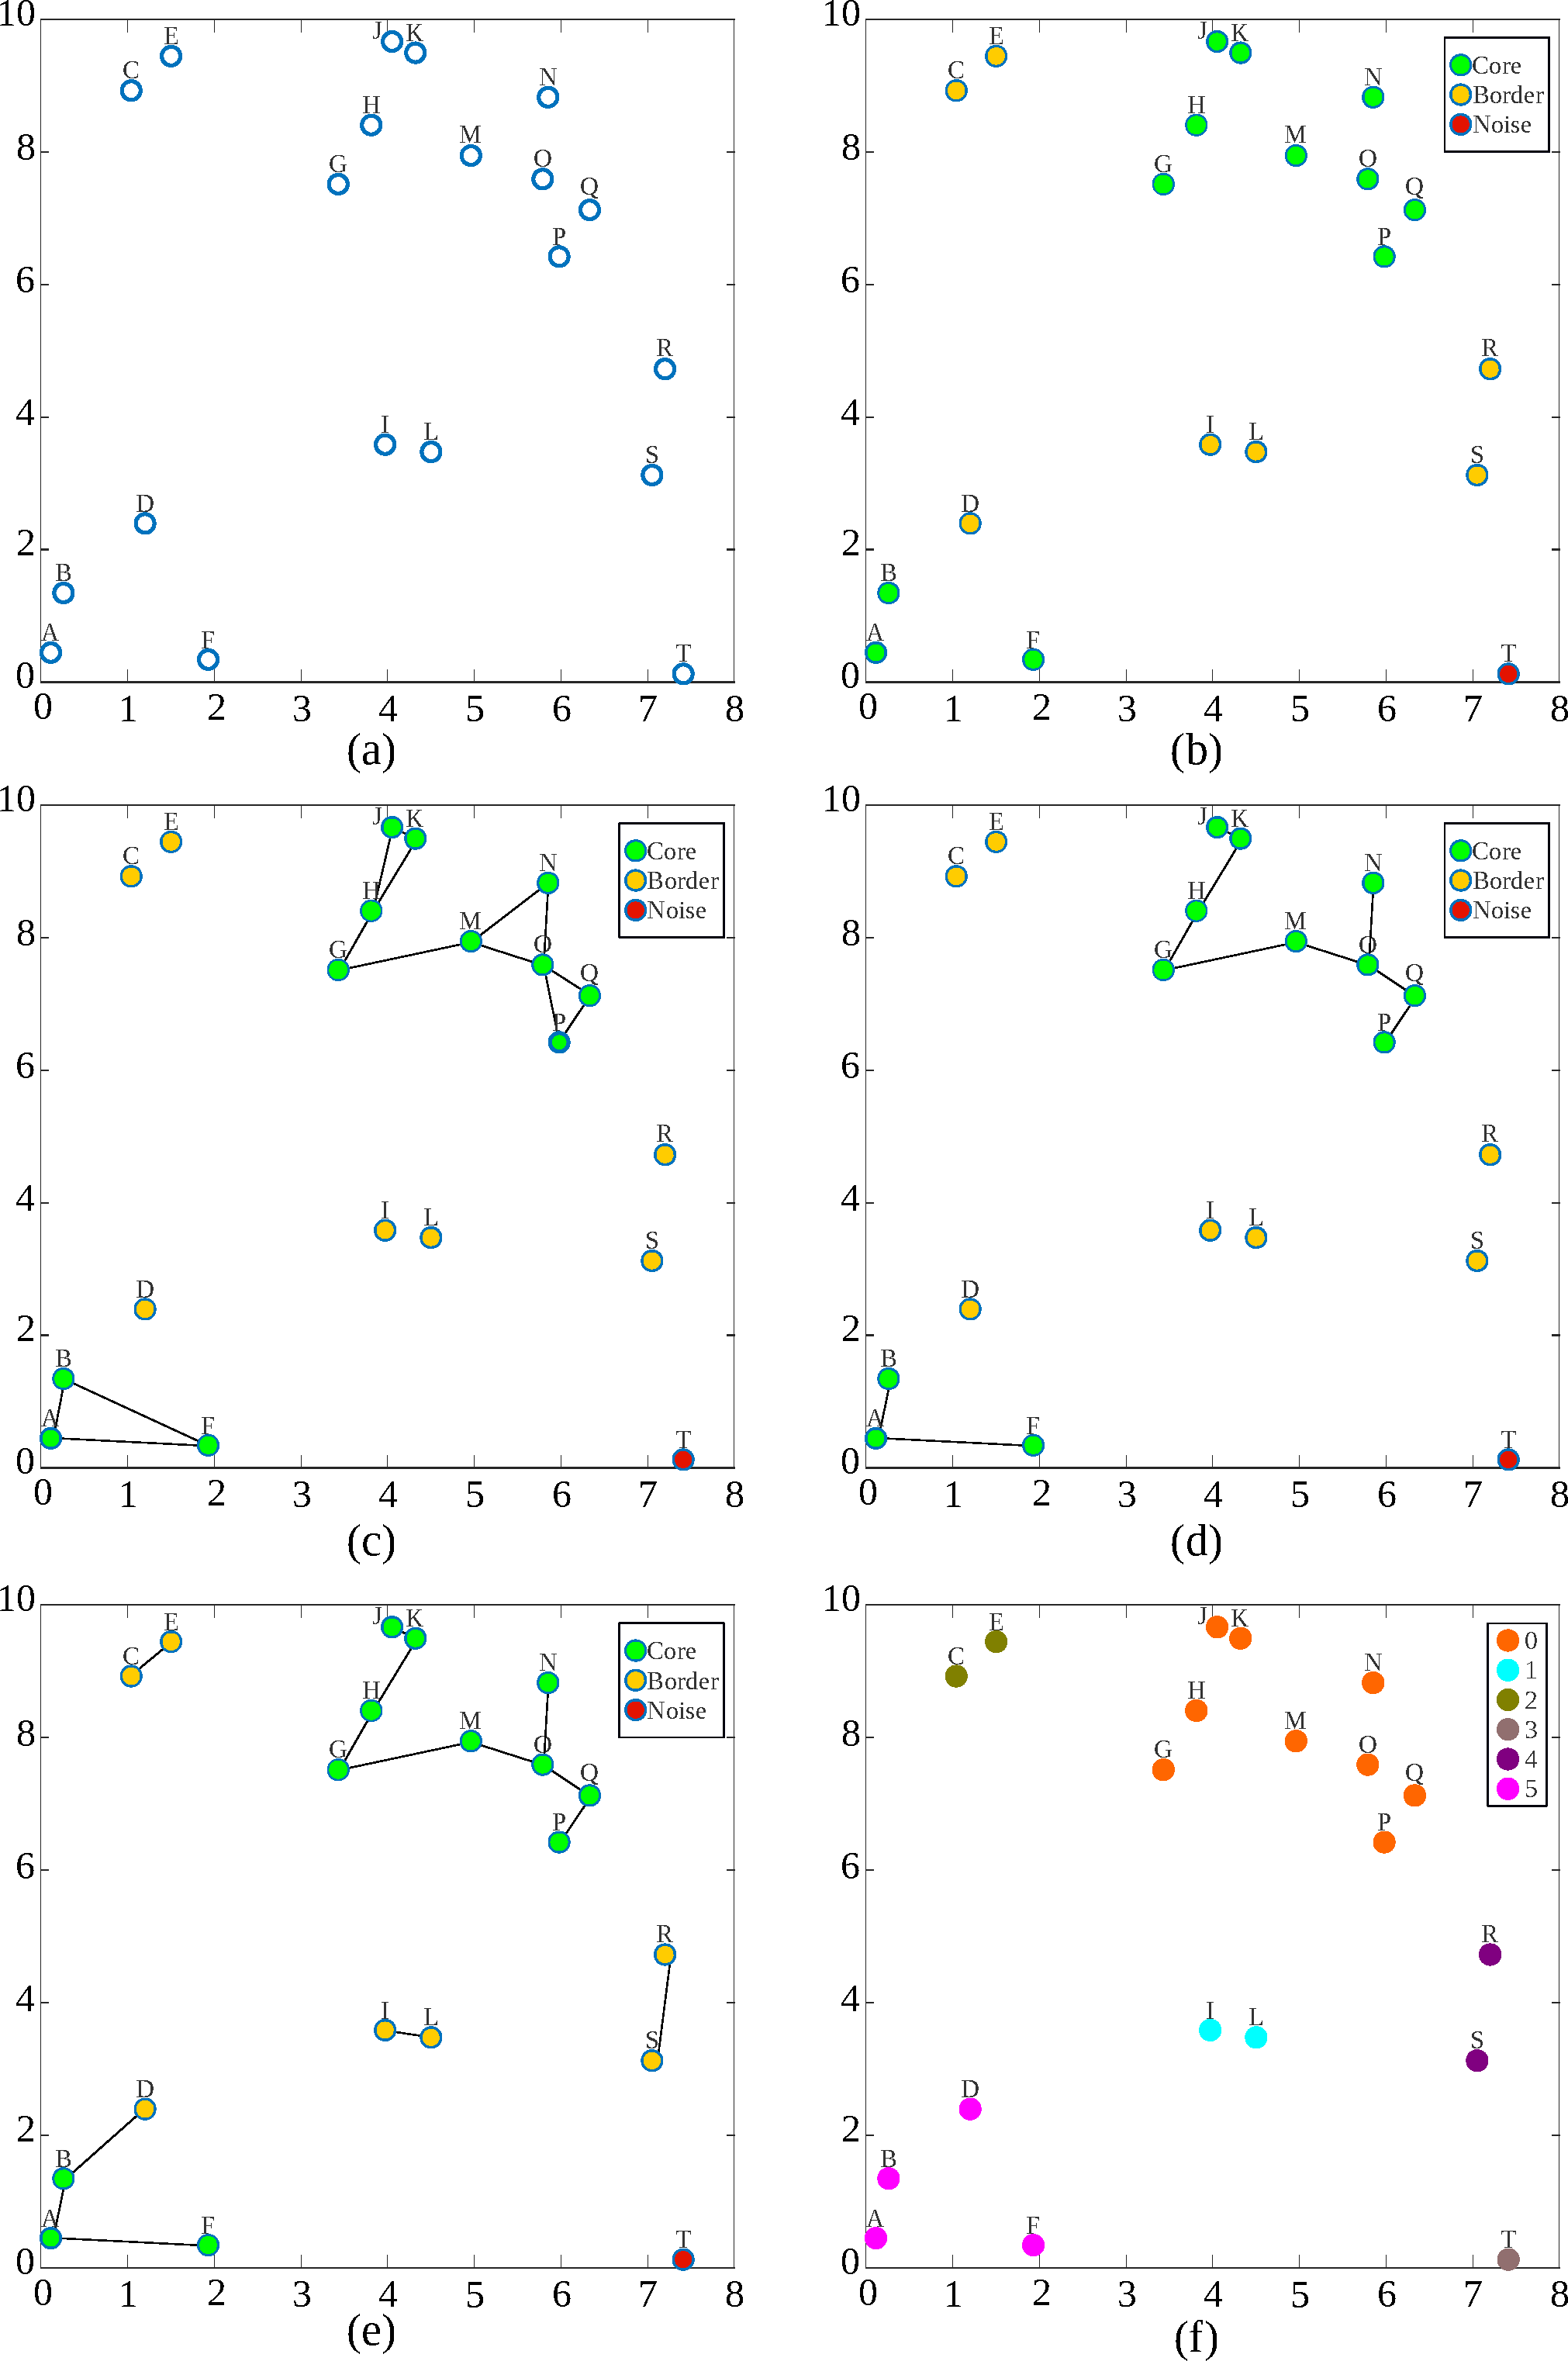
\includegraphics[scale=.41]{_fig/dbscan_passos.pdf}
\caption[Exemplo do algoritmo DBSCAN] {
Exemplo do algoritmo DBSCAN.
(a)~Visualização do conjunto dos dados do exemplo.
(b)~Agrupamento e classificação dos elementos de acordo com número de vizinhos e distância.
(c)~Construção de arestas entre os elementos rotulado como~\textit{Core}.
(d)~Determinação do componente dos elementos~\textit{Core}.
(e)~Agrupamento dos elementos \textit{Border} e \textit{Noise}
(f)~Resultado final do agrupamento.}
\label{fig:ex_dbscan_passos}
\end{figure}


    \item Após a classificação dos elementos, agrupa-se os elementos \textit{Core}.
    O objetivo é construir arestas interligando todos os elementos vizinhos que sejam \textit{Core}.
    A Figura~\ref{fig:ex_dbscan_passos}(c) mostra as arestas para os elementos rotulados com \textit{Core} na Figura~\ref{fig:ex_dbscan_passos}(b) de acordo com os vizinhos descritos na Tabela~\ref{tab:rotulos} que foram obtidos à partir da matriz de distâncias (Tabela~\ref{tab:matriz_distancia}), limiar $\xi = 2$ e número de vizinhos igual a dois. 
    
    \item O próximo passo é gerar componentes os conexos de elementos rotulados como \textit{Core}, sendo uma das possibilidades para a geração desses componentes conexos o uso de árvores geradoras mínimas.
    A Figura~\ref{fig:ex_dbscan_passos}(d) mostra os componentes conexos produzidos para a Figura~\ref{fig:ex_dbscan_passos}(c).
    
    \item Após o agrupamento dos elementos rotulados como \textit{Core}, são analisados os elementos rotulados como \textit{Border}, que são associados ao seu vizinho mais próximo como exemplificado na Figura~\ref{fig:ex_dbscan_passos}(e).
    
    \item O próximo passo é agrupar os elementos rotulados como \textit{Noise}.
    Diversas políticas podem ser empregadas nesse ponto, tais como atribuir cada elemento ``\textit{Noise}'' a um grupo ou agrupá-los todos em um único grupo.
    Nesse trabalho, considera-se a primeira política.
    A Figura~\ref{fig:ex_dbscan_passos}(e) mostra os elementos \textit{Noise} da Figura~\ref{fig:ex_dbscan_passos}(b) como grupos unitários.
    
    \item Finalmente, o DBSCAN realiza a substituição dos rótulos iniciais por rótulos dos grupos, onde todos os elementos conectados pelo mesmo caminho serão agrupados em um mesmo \textit{cluster} e as arestas descartadas.
    O resultado final do método DBSCAN para o exemplo da Figura~\ref{fig:ex_dbscan_passos}(a) é mostrado na Figura~\ref{fig:ex_dbscan_passos}(f).
    
\end{enumerate}


\subsection{Trabalhos relacionados} 

Os conceitos revisados até aqui são usados extensivamente nos trabalhos da literatura que abordam o contexto de diagnóstico de úlceras em membros inferiores, de acordo com diversos pesquisadores.
Em particular, o trabalho de \citeonline{Dorileo2008} aborda a importância da padronização das amostras de úlceras em um modelo de cores.
\citeonline{Bedo2015a} utilizam o paradigma supervisionado para o diagnóstico das imagens levantadas por \citeonline{Dorileo2008} e realizam um comparativo entre as características das imagens, a fim de apresentar a melhor forma para classificar imagens de úlceras.

\citeonline{Godeiro2018} utilizam uma redução de espaço de cor para a extração de regiões feridas de acordo com seus tecidos mais dominantes.
\citeonline{Mukherjee2014} aplicam extratores de cores de baixo nível para transformar partes da imagem em pontos multidimensionais e aplica o classificador SVM para a rotular feridas crônicas.
\citeonline{Blanco2016} usam o conjunto de dados de \citeonline{Dorileo2008}, mas aplicam uma estratégia de divisão e conquista na qual as feridas são segmentadas com o apoio de métodos de construção de superpixels SLIC e os superpixels são representados em espaços de múltiplas dimensões por descritores MPEG-7~\cite{Blanco2016}.
Já \citeonline{Chino2018} utilizam o classificador RandomForest e o extrator ``Bag-of-Signatures''.
Por último \citeonline{Nejati2018} usam características oriundas de redes neurais de aprendizado profundo e o classificador SVM. 

\begin{table}[!htb]
\centering
\caption[Trabalhos relacionados revisados]{Trabalhos relacionados revisados.}
\begin{tabular}{c|c|c|c}
\hline
\rowcolor[HTML]{C0C0C0} 
{\color[HTML]{000000} \textbf{Autor \& Ano}} & {\color[HTML]{000000} \textbf{Extrator de característica}} & {\color[HTML]{000000} \textbf{Classificador}} & {\color[HTML]{000000} \textbf{Precisão}} \\ \hline
{\color[HTML]{000000} \citeonline{Pereyra2014} } & {\color[HTML]{000000} Matrizes de co-ocorrência de cor} & {\color[HTML]{000000} kNN} & {\color[HTML]{000000} $75,00\%$} \\ \hline
\rowcolor[HTML]{EFEFEF} 
{\color[HTML]{000000} \citeonline{Blanco2016} } & {\color[HTML]{000000} 3S-Measure} & {\color[HTML]{000000} \textit{RandomForest}} & {\color[HTML]{000000} $86,81\%$} \\ \hline
{\color[HTML]{000000} \citeonline{Chino2018} } & {\color[HTML]{000000} Nenhum} & {\color[HTML]{000000} \textit{RandomForest} } & {\color[HTML]{000000} $89,00\%$ } \\ \hline
\rowcolor[HTML]{EFEFEF}
{\color[HTML]{000000} \citeonline{Nejati2018}} & {\color[HTML]{000000} AlexNet e ImageNet} & {\color[HTML]{000000} \textit{SVM} } & {\color[HTML]{000000} $86,40\%$ } \\ \hline
\end{tabular}
\end{table}

\subsection{Conclusões parciais}

Esse trabalho consiste no estudo e implementação de técnicas computacionais de processamento de imagens e aprendizado de máquina.
Portanto, espera-se tirar proveito dos resultados e avanços relatados em trabalhos anteriores, para identificar e segmentar as imagens de úlceras em membros inferiores.
Nesse sentido, técnicas clássicas de processamento de imagens são úteis para auxiliar e melhorar os resultados da segmentação entre o fundo da imagem e lesão.
Essa separação pode ser finalizada por uma tarefa de limiarização ou classificação.
Outra abordagem a ser avaliada na sequência é distinguir entre grupos, ou tecidos, dentro da lesão em si.
A literatura traz relatos do uso eficiente de métodos de superpixel para essa etapa.

Uma vez que seja possível dividir a lesão em \textit{superpixels} candidatos, estas regiões, com o valor médio do superpixel em espaço de cor adequado, podem ser agrupadas por um algoritmo particional, como o DBSCAN.
Conclui-se que separar planos de fundos de pele e, depois disso, distinguir os tipos de tecidos envolvidos com a caracterização de úlceras em membros inferiores requer combinar várias, senão todas, as técnicas revisadas nessa seção.
\newpage
\thispagestyle{plain} % empty
\mbox{}
